% ATTENZIONE: Nei file secondari NON devi inserire \begin{document} o \end{document}.
\newpage

\chapterimage{Pictures/Indice.png}
\chapter{Attention Mechanisms and Transformer Networks}\label{ch:attention_transformers}

\section{Introduction: Transcending the Recurrent Bottleneck}

In Chapter~\ref{ch:sequence_models}, we explored sequential modeling through the lens of recurrence. While architectures such as Long Short-Term Memory (LSTM) alleviate the vanishing gradient problem via an additive cell state highway, recurrent systems remain fundamentally constrained by their temporal formulation:

\begin{enumerate}[leftmargin=*]
    \item \textbf{The Information Bottleneck:} In standard sequence-to-sequence networks, the encoder squashes an arbitrary-length input sequence $\{x_1, \dots, x_T\}$ into a single fixed-dimensional bottleneck vector $c = h_T$. As sequence length grows ($T \ge 30$), compressing rich sentence context into a static vector causes catastrophic information loss.
    \item \textbf{Sequential Computational Dependency ($O(n)$):} Recurrent computations are strictly serialized across time: hidden state $h_t$ cannot be computed until $h_{t-1}$ is fully evaluated. Consequently, training cannot be parallelized across sequence length on modern hardware accelerators.
    \item \textbf{Linear Interaction Path Length ($O(n)$):} Information transfer between distant tokens must propagate step-by-step through intermediate hidden states, increasing susceptibility to signal attenuation and gradient decay.
\end{enumerate}

This chapter details the paradigm shift that overcame these structural limits: the invention of the \textbf{Attention Mechanism} and the emergence of the \textbf{Transformer} architecture, based on the course lecture modules by Prof.~Fabio Galasso~\cite{galasso2025seqmodels2}.


\section{From Recurrence to Attention}

\subsection{The Information Bottleneck in Vanilla Seq2Seq}

As formalized by Sutskever et al.~\cite{sutskever2014sequence}, a standard Sequence-to-Sequence (Seq2Seq) model maps an input sequence $x = (x_1, \dots, x_T)$ into an output sequence $y = (y_1, \dots, y_{T'})$ using an Encoder-Decoder framework:
\begin{align}
    h_t &= f_W(x_t, h_{t-1}) \quad &\text{(Encoder)} \\
    s_t &= g_U(y_{t-1}, s_{t-1}, c) \quad &\text{(Decoder)}
\end{align}
where:
\begin{itemize}[leftmargin=*]
    \item $f_W$ denotes the recurrent transition function of the encoder (e.g.\@ an RNN, LSTM, or GRU cell) parameterized by its collection of learnable weights $W$.
    \item $g_U$ denotes the recurrent transition function of the decoder, parameterized by its own set of learnable weights $U$.
    \item $c = h_T$ is the static context vector passed from the final encoder step to the decoder.
\end{itemize}
When translating long documents ($T \ge 30$), forcing the entire semantic representation of the source sentence through the single fixed-dimensional vector $h_T$ constitutes an unsustainable \textbf{information bottleneck}.

\subsection{The Bahdanau Additive Attention Mechanism}

To resolve this limitation, Bahdanau et al.~\cite{bahdanau2015neural} introduced the \textbf{Attention Mechanism}. Rather than relying on a static context vector, the decoder dynamically computes a \textbf{customized context vector $c_t$} at every decoding time step $t$, as illustrated in Figure~\ref{fig:seq2seq_attention_unrolled}.

\begin{figure}[htbp]
    \centering
    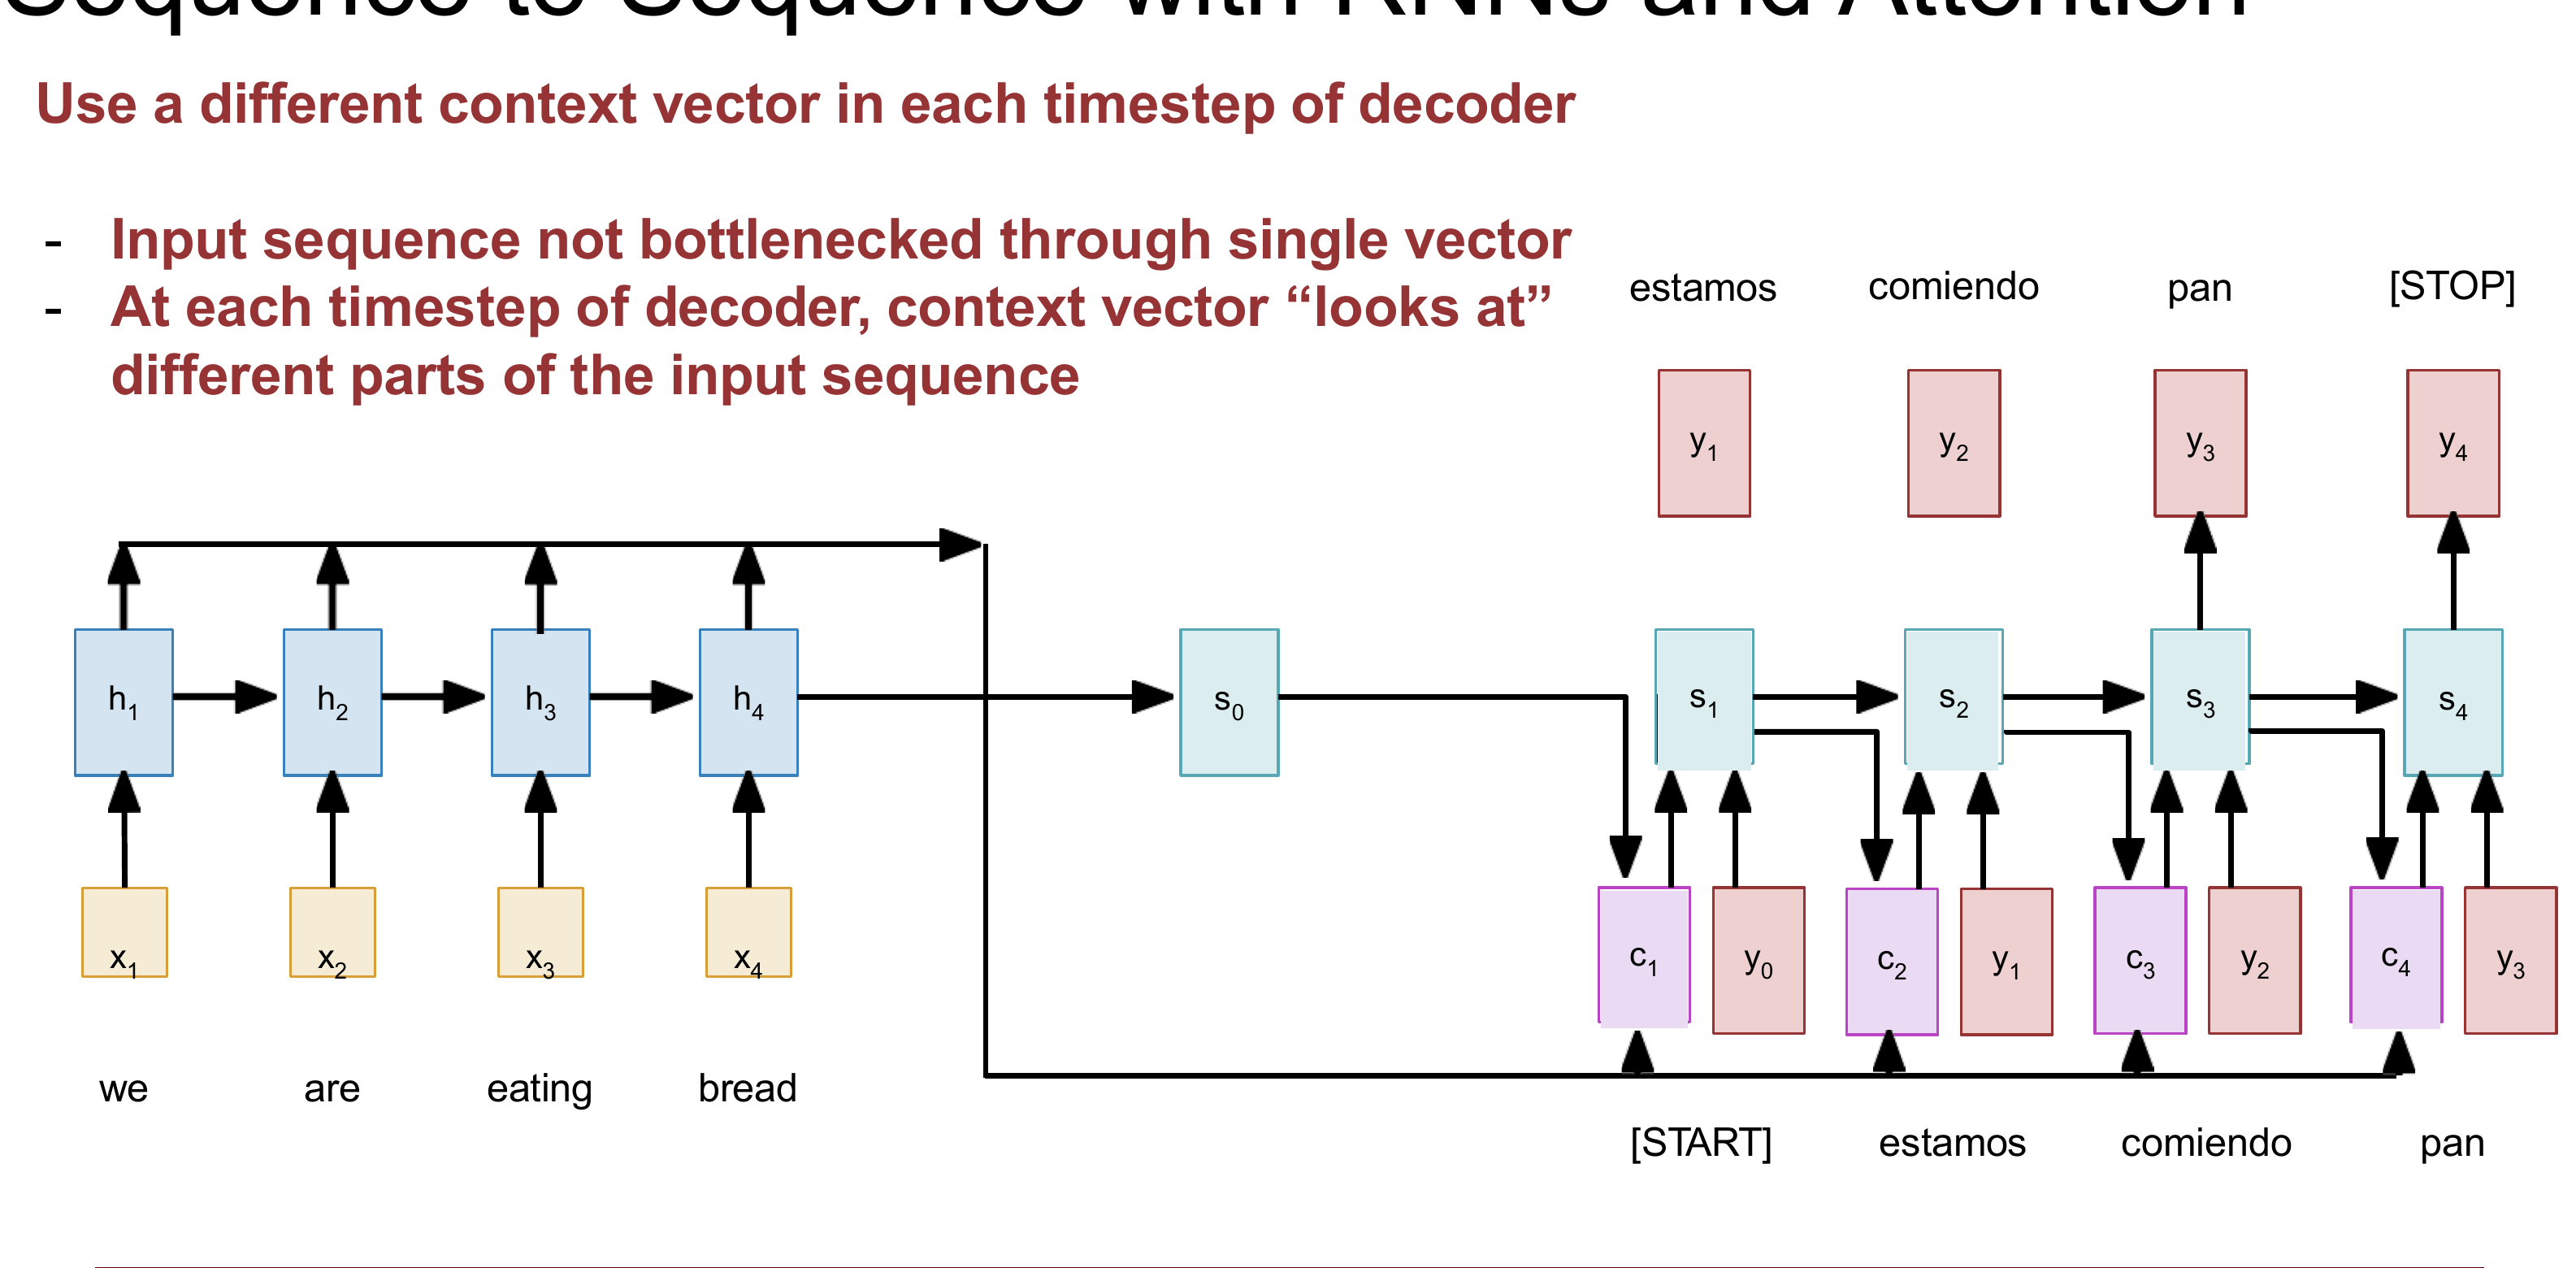
\includegraphics[width=0.95\textwidth]{Pictures/seq2seq_attention_unrolled.png}
    \caption{Unrolled Sequence-to-Sequence architecture with dynamic attention (from course slides~\cite{galasso2025seqmodels2}). At each decoding step $t$, the decoder generates a customized context vector $c_t$ that selectively attends to different parts of the input sequence.}\label{fig:seq2seq_attention_unrolled}
\end{figure}

The attention mechanism operates via four sequential steps:

\begin{enumerate}[leftmargin=*]
    \item \textbf{Alignment Scores ($e_{t,i}$):} The model evaluates how well the current decoder state $s_{t-1}$ matches each encoder hidden state $h_i$:
    \begin{equation}
        e_{t,i} = f_{\text{att}}(s_{t-1}, h_i)
    \end{equation}
    where $f_{\text{att}}$ is parameterized as a small feed-forward Multi-Layer Perceptron (MLP) trained jointly with the rest of the network.
    
    \item \textbf{Attention Weights ($\alpha_{t,i}$):} The scalar alignment scores are normalized across all input positions $i \in \{1, \dots, T\}$ via a Softmax operation:
    \begin{equation}
        \alpha_{t,i} = \frac{\exp(e_{t,i})}{\sum_{k=1}^T \exp(e_{t,k})}, \quad \text{such that } 0 < \alpha_{t,i} < 1 \text{ and } \sum_{i=1}^T \alpha_{t,i} = 1
    \end{equation}
    The weight $\alpha_{t,i}$ represents the probability or relative importance assigned to input token $x_i$ when generating output word $y_t$.
    
    \item \textbf{Dynamic Context Vector ($c_t$):} The context vector is computed as a weighted average over all encoder hidden states:
    \begin{equation}
        c_t = \sum_{i=1}^T \alpha_{t,i} h_i
    \end{equation}
    
    \item \textbf{Decoder Recurrent Update:} The new decoder state and output token probabilities are computed conditioning on $c_t$:
    \begin{equation}
        s_t = g_U(y_{t-1}, s_{t-1}, c_t), \quad P(y_t \mid y_{<t}, x) = \operatorname{softmax}(W_v s_t)
    \end{equation}
\end{enumerate}

\begin{Notebox}
\textbf{End-to-End Differentiability:}
Every operation in the attention formulation (affine projections, Softmax, weighted averaging) is fully differentiable. No explicit target supervision is needed for the attention weights $\alpha_{t,i}$: backpropagation through the cross-entropy translation loss trains the attention mechanism to discover linguistic alignments automatically.
\end{Notebox}

\subsection{\texorpdfstring{Step-by-Step Walkthrough: Dynamic Alignment at Decoding Step $t=2$}{Step-by-Step Walkthrough: Dynamic Alignment at Decoding Step t=2}}

To fully appreciate the operational mechanics of the attention mechanism, we trace the concrete translation example presented by Prof.\@ Galasso~\cite{galasso2025seqmodels2}, based on Bahdanau et al.~\cite{bahdanau2015neural}: translating the English sentence \textit{“we are eating bread”} into Spanish (\textit{“estamos comiendo pan”}).

Figure~\ref{fig:bahdanau_step2_example} details the exact state of the network at decoding step $t=2$, where the model generates the target word \textit{“comiendo”}.

\begin{figure}[htbp]
    \centering
    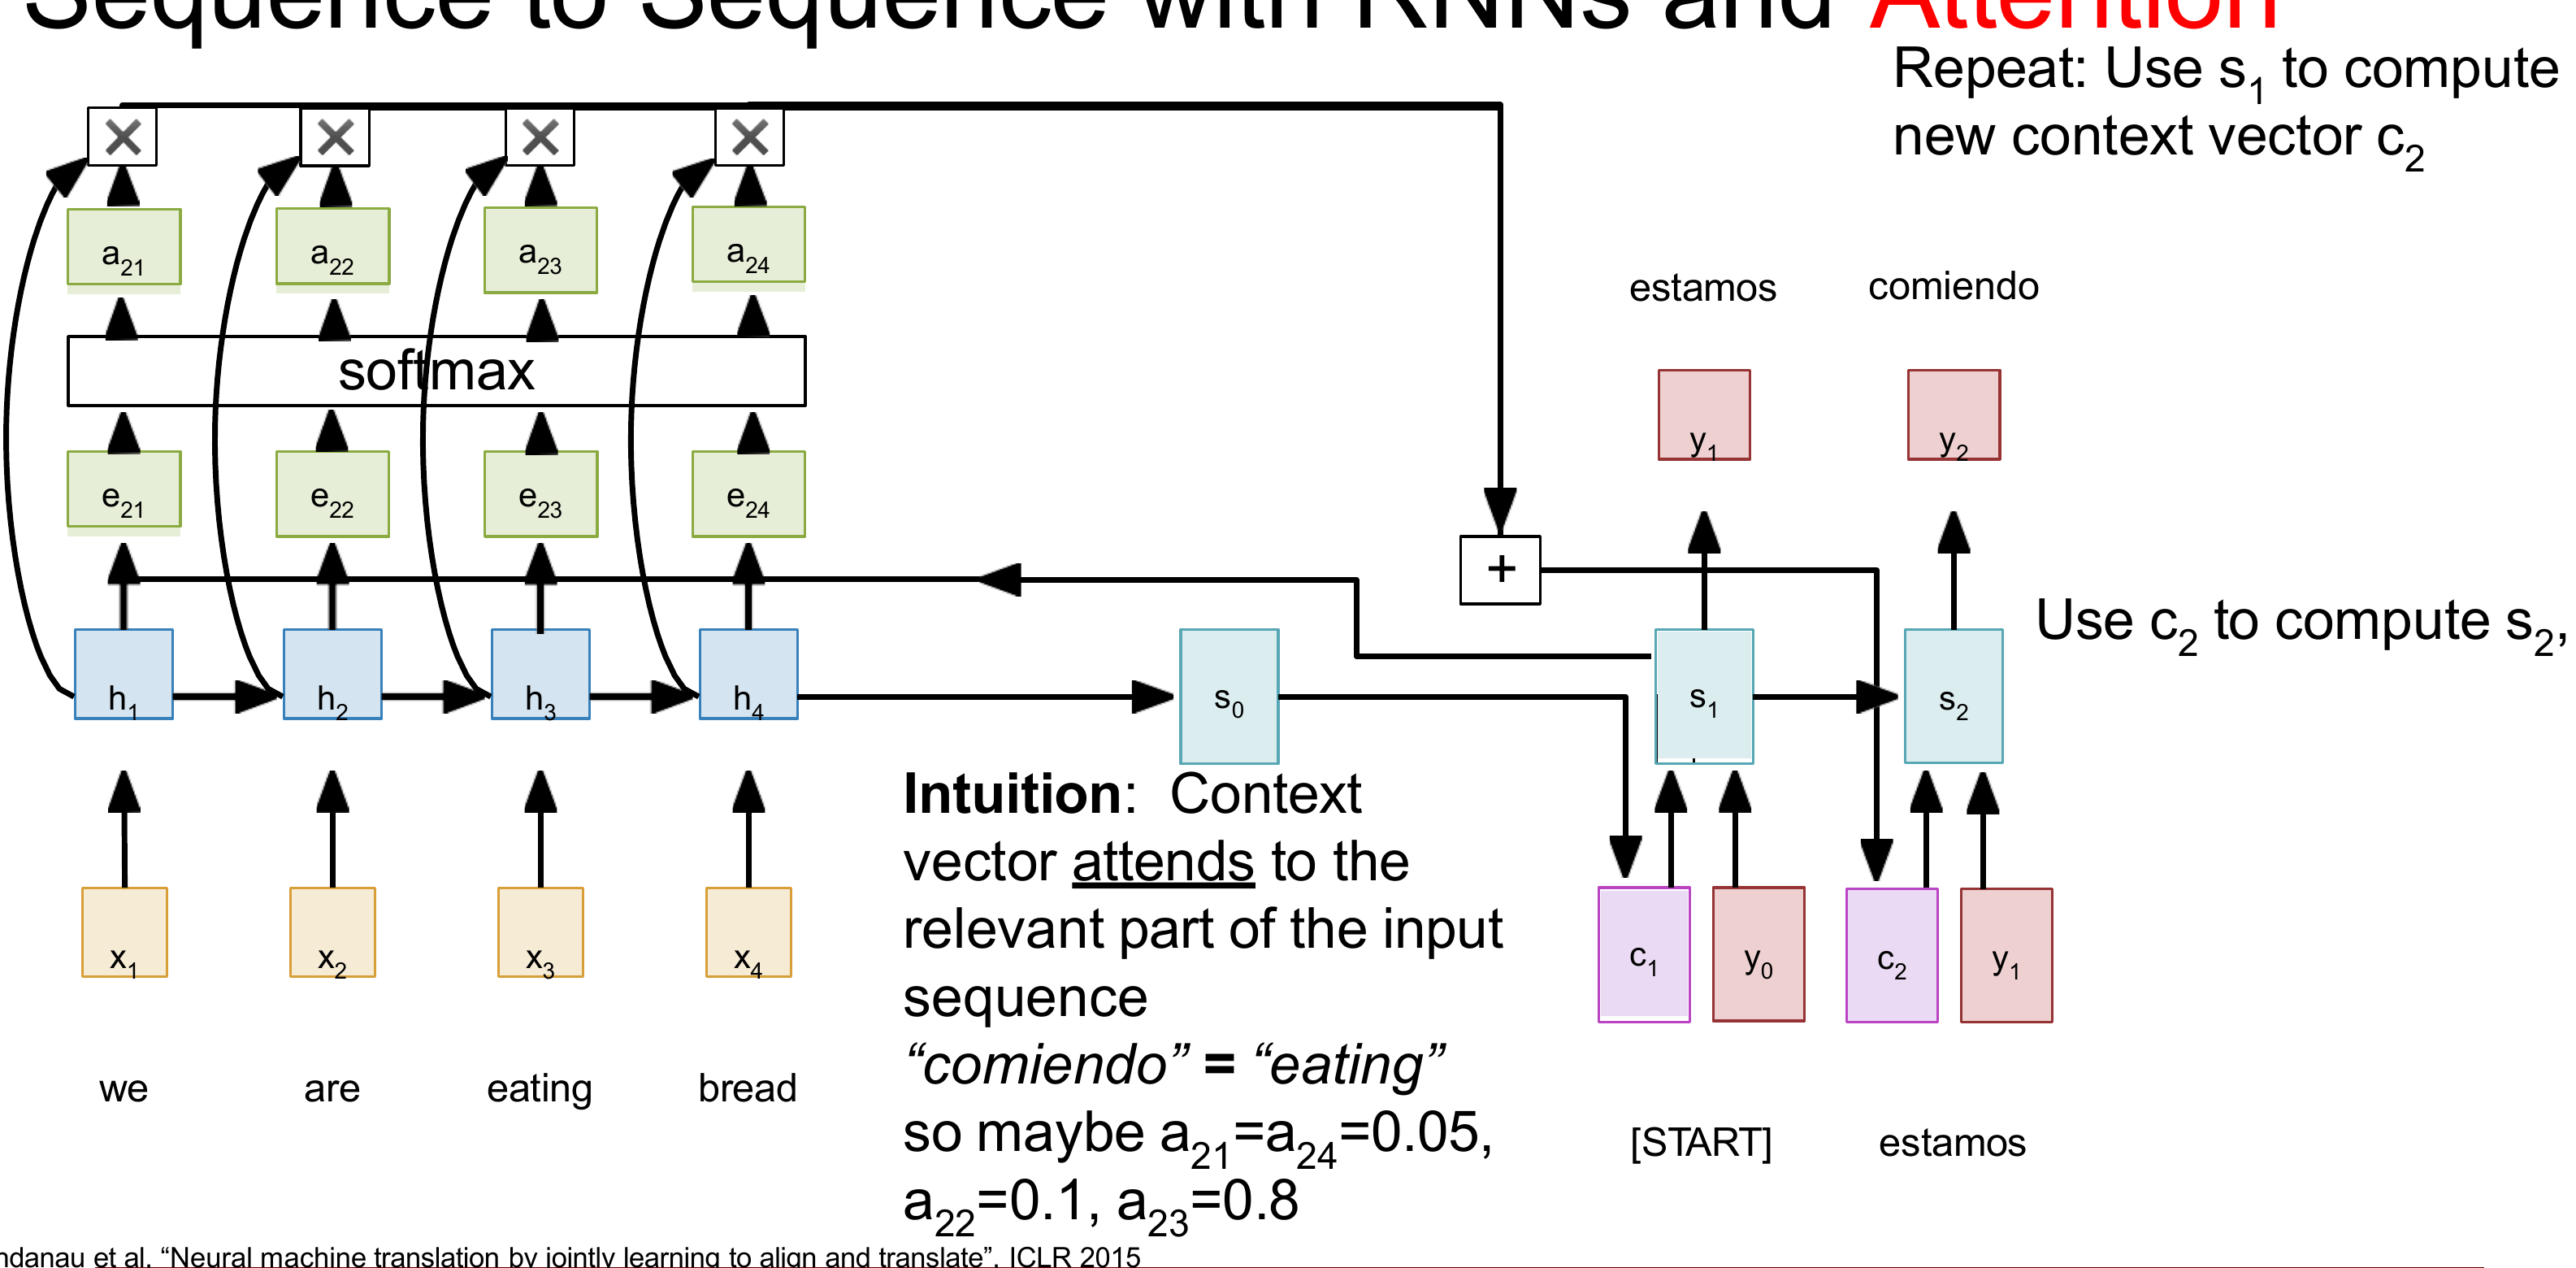
\includegraphics[width=0.92\textwidth]{Pictures/bahdanau_attention_step_example.png}
    \caption{Detailed walkthrough of the Attention mechanism at decoding step $t=2$ (from course slides~\cite{galasso2025seqmodels2, bahdanau2015neural}). The decoder utilizes hidden state $s_1$ to evaluate alignment scores across all encoder hidden states $h_1, \dots, h_4$. After Softmax normalization, the model concentrates $80\%$ of its attention weight on $h_3$ (\textit{“eating”}), synthesizing context vector $c_2$ to predict $y_2 =$ \textit{“comiendo”}.}\label{fig:bahdanau_step2_example}
\end{figure}

The decoding step unfolds across five distinct computational stages:

\begin{enumerate}[leftmargin=*]
    \item \textbf{Source Encoding ($T_x = 4$):}
    The input tokens $x_1 =$ \textit{“we”}, $x_2 =$ \textit{“are”}, $x_3 =$ \textit{“eating”}, and $x_4 =$ \textit{“bread”} are processed sequentially by the recurrent encoder, generating contextual hidden states $h_1, h_2, h_3, h_4 \in \mathbb{R}^d$. Crucially, unlike vanilla Seq2Seq, \textbf{all four hidden states are retained in memory} throughout the decoding phase.

    \item \textbf{Decoder Prior State at Step $t=1$:}
    At step $t=1$, the decoder received the initial start token $y_0 = \texttt{[START]}$ and initial context $c_1$. It generated the first Spanish token $y_1 =$ \textit{“estamos”} (translating the subject and auxiliary verb \textit{“we are”}), updating its recurrent hidden state to $s_1$. State $s_1$ now encodes the working memory that the plural first-person continuous subject has been established and an active verb is required next.

    \item \textbf{Querying Encoder States via Alignment Scores ($e_{2, i}$):}
    To discover which English word corresponds to the upcoming action, decoder state $s_1$ acts as a \textbf{query} against each encoder state $h_i$:
    \begin{equation}
        e_{2, i} = f_{\text{att}}(s_1, h_i) = v_a^\top \tanh(W_a s_1 + U_a h_i), \quad \text{for } i \in \{1, 2, 3, 4\}
    \end{equation}
    The feed-forward scoring network evaluates the semantic compatibility between what the decoder needs next ($s_1$) and what each source position represents ($h_i$).

    \item \textbf{Softmax Normalization and Weight Distribution ($\alpha_{2, i}$):}
    The raw scalar alignment scores are exponentiated and normalized via Softmax to yield a strict probability distribution:
    \begin{equation}
        \alpha_{2, i} = \frac{\exp(e_{2, i})}{\sum_{k=1}^4 \exp(e_{2, k})}
    \end{equation}
    As highlighted in the course slides, the learned weights reflect the underlying linguistic correspondence:
    \begin{itemize}[leftmargin=*]
        \item $\alpha_{2, 1} = 0.05$ (weight assigned to \textit{“we”})
        \item $\alpha_{2, 2} = 0.10$ (weight assigned to \textit{“are”})
        \item $\mathbf{\alpha_{2, 3} = 0.80}$ (\textbf{dominant attention concentrated on \textit{“eating”}})
        \item $\alpha_{2, 4} = 0.05$ (weight assigned to \textit{“bread”})
    \end{itemize}
    Because the model must produce the Spanish gerund \textit{“comiendo”}, the alignment network concentrates $80\%$ of the probability mass directly on token $x_3$ (\textit{“eating”}).

    \item \textbf{Dynamic Context Synthesis ($c_2$) and the Recurrent Update Function $g_U$:}
    The customized context vector $c_2$ is synthesized as the weighted linear combination:
    \begin{equation}
        c_2 = 0.05 \, h_1 + 0.10 \, h_2 + \mathbf{0.80 \, h_3} + 0.05 \, h_4 \;\approx\; h_3
    \end{equation}
    Vector $c_2$ functions as a soft, differentiable spotlight: irrelevant past tokens (\textit{“we”, “are”}) and future objects (\textit{“bread”}) are heavily suppressed, channeling pure semantic information about the eating action into the decoder. 

    The decoder state is then updated via the recurrent transition operator:
    \begin{equation}
        s_2 = g_U(y_1, s_1, c_2)
    \end{equation}
    To understand the concrete mechanics of $g_U$, note that it integrates three distinct sources of information:
    \begin{itemize}[leftmargin=*]
        \item $y_1$: The embedding of the previously generated token (\textit{“estamos”}).
        \item $s_1$: The previous recurrent hidden state (carrying decoder past history).
        \item $c_2$: The dynamic context vector synthesized by the attention mechanism.
    \end{itemize}
    If the decoder is implemented as a standard recurrent layer, the transition function $g_U$ expands explicitly as:
    \begin{equation}
        s_2 = \tanh\Big( \underbrace{U_{ss} \, s_1}_{\text{previous state}} + \underbrace{U_{ys} \, y_1}_{\text{previous token}} + \underbrace{U_{cs} \, c_2}_{\text{attention context}} + b_U \Big)
    \end{equation}
    where $U = \{U_{ss}, U_{ys}, U_{cs}, b_U\}$ denotes the collection of learnable projection matrices and bias terms of the decoder cell. In gated implementations (such as the Gated Recurrent Unit used by Bahdanau et al.), $g_U$ represents the gate equations (reset and update gates) operating over the concatenated vector $[y_1; s_1; c_2]$.

    Conditioned on the updated state $s_2$, the linear vocabulary head projects $s_2$ through Softmax to emit:
    \begin{equation}
        y_2 = \text{\textit{“comiendo”}}
    \end{equation}
\end{enumerate}

\begin{InsightBox}
\textbf{Why Vanilla Seq2Seq Fails Where Attention Succeeds:} \\
In a vanilla Seq2Seq network without attention, the decoder at step $t=2$ would have access only to the static bottleneck vector $c = h_4$ (the state produced after processing \textit{“bread”}). Because $h_4$ is separated from \textit{“eating”} by subsequent recurrent steps, its representation suffers from recency bias and information decay. The decoder is forced to remember the entire sentence structure from a single vector.

With attention, the model bypasses temporal distance entirely: at time step $t=2$, it establishes a direct, $\mathcal{O}(1)$ highway straight to $h_3$, retrieving the exact information needed without memory degradation.
\end{InsightBox}

\newpage
\subsection{Interpreting Attention Matrices and Word Reordering}

A remarkable consequence of the attention mechanism is its intrinsic interpretability. By visualizing the matrix of attention weights $\alpha_{t,i} \in \mathbb{R}^{T' \times T}$, one can directly observe how the model aligns source and target tokens, as shown in Figure~\ref{fig:attention_weights_matrix}.

\begin{figure}[htbp]
    \centering
    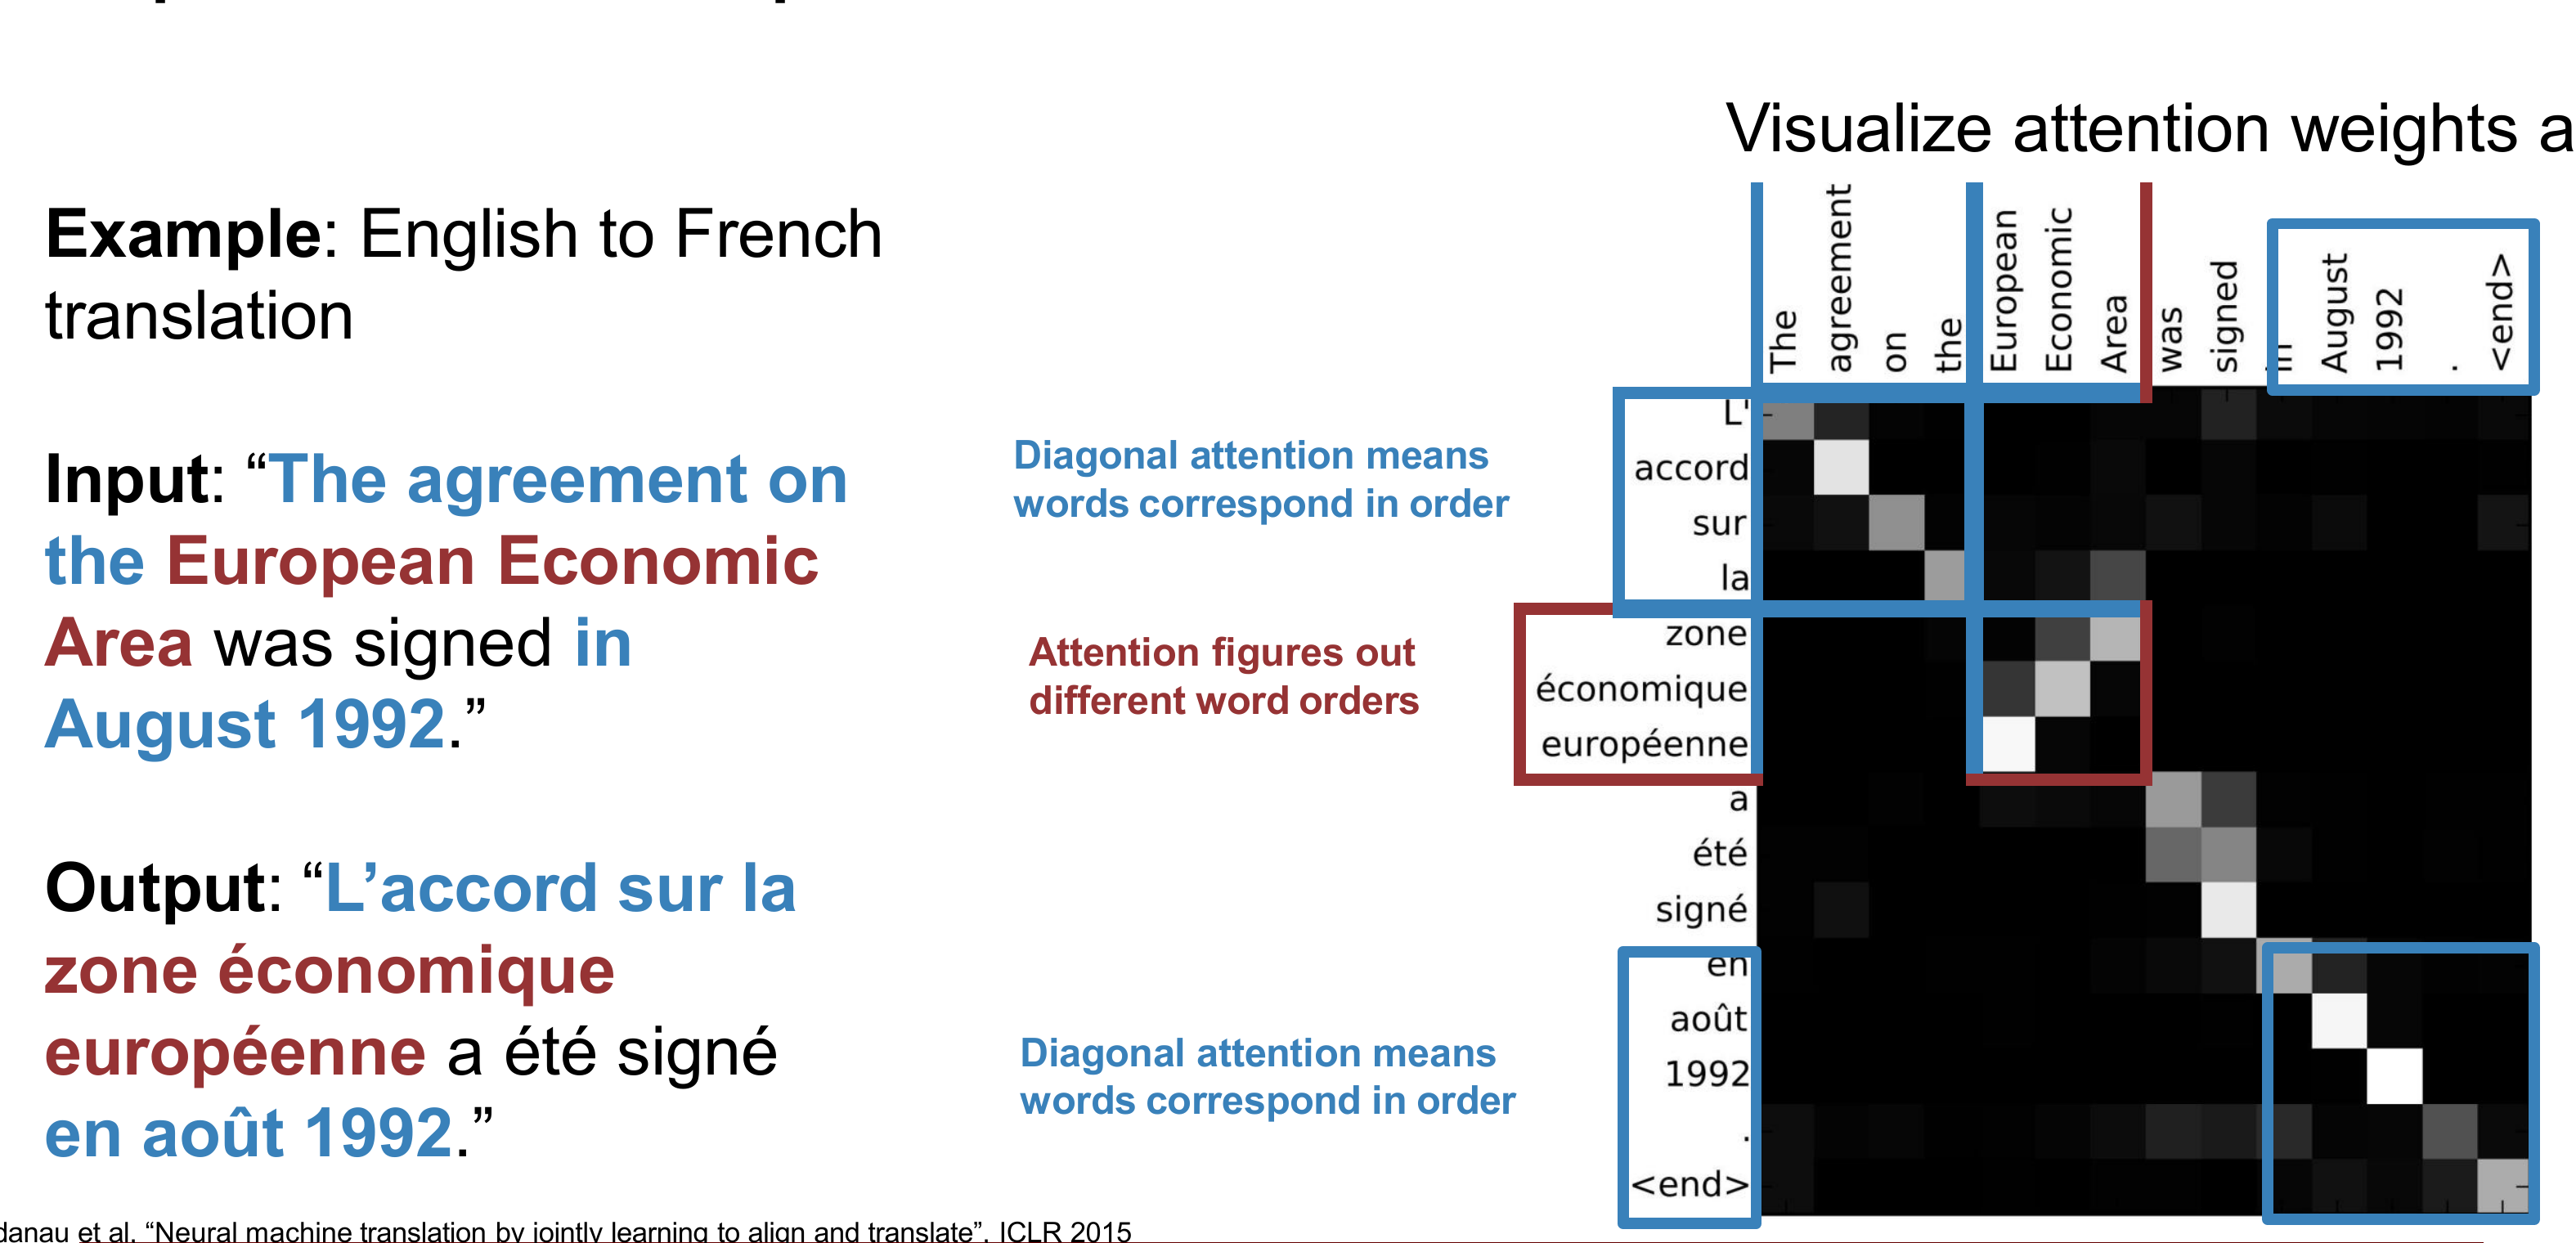
\includegraphics[width=0.82\textwidth]{Pictures/attention_weights_matrix.png}
    \caption{Visualization of attention alignment weights for English-to-French translation (Bahdanau et al.~\cite{bahdanau2015neural}, from course slides). Strong diagonal values indicate sequential correspondence, while off-diagonal elements show grammatical word reordering.}\label{fig:attention_weights_matrix}
\end{figure}

\begin{keywordbox}
\textbf{Monotonic Alignments versus Non-Monotonic Reordering} \\
As illustrated in the attention matrix of Figure~\ref{fig:attention_weights_matrix}, when languages share syntactic ordering, attention concentrates along the main diagonal. However, when syntactic structures differ (e.g., English \textit{“European Economic Area”} $\longrightarrow$ French \textit{“zone {\'e}conomique europ{\'e}enne”}), the attention matrix exhibits an off-diagonal transpose: the model correctly looks ahead to translate \textit{“zone”} before returning to attend to \textit{“{\'e}conomique”} and \textit{“europ{\'e}enne”}.
\end{keywordbox}

\begin{InsightBox}
\textbf{The Unordered Set Property (Slide 27):} \\
Notice an unexpected theoretical property of the attention decoder: it does not rely on the fact that the encoder vectors $h_i$ form a temporally ordered sequence. The decoder treats them purely as an \textbf{unordered set of feature vectors} $\{h_i\}$!

This insight proves revolutionary: because attention operates over arbitrary unordered sets, the same mechanism can be directly applied to sets of spatial image features, audio tokens, or graph nodes.
\end{InsightBox}

\subsection{Spatial Attention in Computer Vision: Show, Attend and Tell}

Xu et al.~\cite{xu2015show} generalized Bahdanau's sequence attention to multi-modal computer vision in the celebrated \textit{“Show, Attend and Tell”} architecture, illustrated in Figure~\ref{fig:show_attend_tell_grid}.

\begin{figure}[htbp]
    \centering
    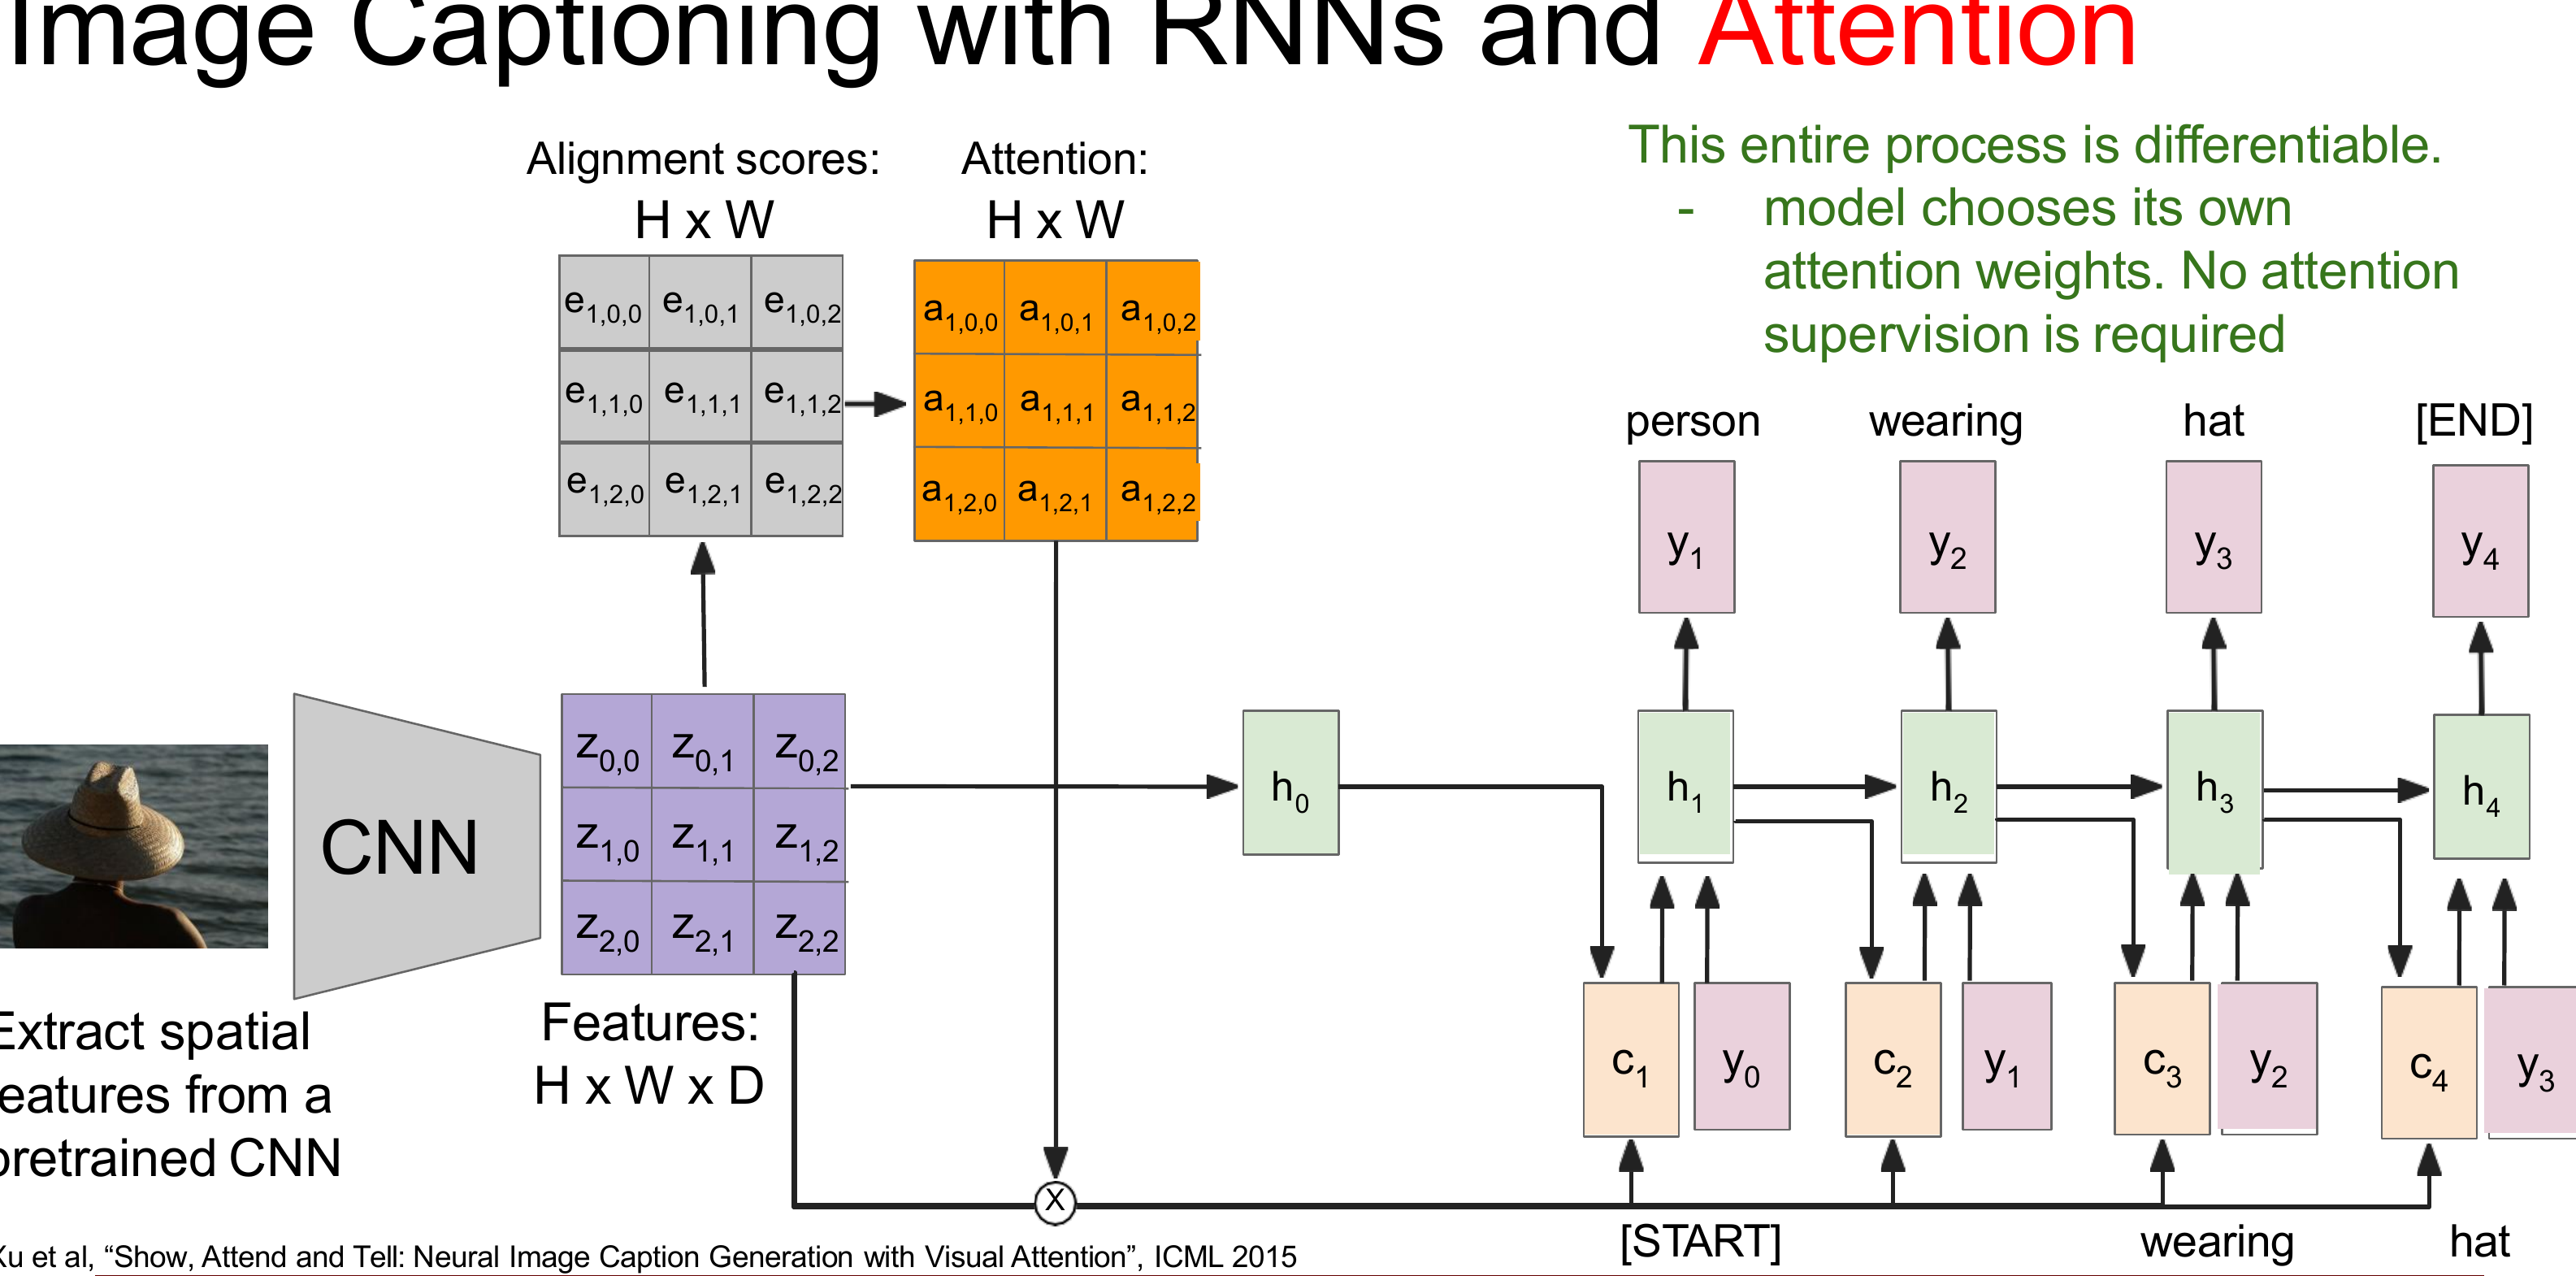
\includegraphics[width=0.92\textwidth]{Pictures/show_attend_tell_grid.png}
    \caption{Image captioning with spatial 2D visual attention (Xu et al.~\cite{xu2015show}, from course slides). Instead of a single image vector, the decoder computes 2D attention maps over a grid of spatial feature vectors $z_{i,j}$, dynamically focusing on salient image regions for each word.}\label{fig:show_attend_tell_grid}
\end{figure}

Rather than extracting a single global vector (such as \texttt{FC-4096} from VGG in Chapter~\ref{ch:sequence_models}), a convolutional backbone extracts a 3D spatial tensor of feature vectors $z \in \mathbb{R}^{H \times W \times D}$. At each time step $t$:
\begin{enumerate}[nosep, leftmargin=*]
    \item Scalar alignment scores are computed across the 2D grid: $e_{t, i, j} = f_{\text{att}}(h_{t-1}, z_{i, j})$.
    \item Spatial attention weights are computed via 2D Softmax: $\alpha_{t, i, j} = \frac{\exp(e_{t, i, j})}{\sum_{u, v} \exp(e_{t, u, v})}$.
    \item A localized visual context vector is accumulated: $c_t = \sum_{i=1}^H \sum_{j=1}^W \alpha_{t, i, j} z_{i, j}$.
\end{enumerate}
As the decoder outputs words sequentially (\textit{“person”} $\longrightarrow$ \textit{“wearing”} $\longrightarrow$ \textit{“hat”}), the attention maps visibly shift their spatial focus across the corresponding regions of the input image.


\section{Self-Attention and Scaled Dot-Product Mechanics}

\subsection{From General Attention to Self-Attention}

While standard attention computes interactions between two distinct sequences (decoder states querying encoder states), \textbf{Self-Attention} computes interactions between elements within the \textbf{same} sequence. Each token is updated by comparing itself against all other tokens in the input.

\begin{figure}[htbp]
    \centering
    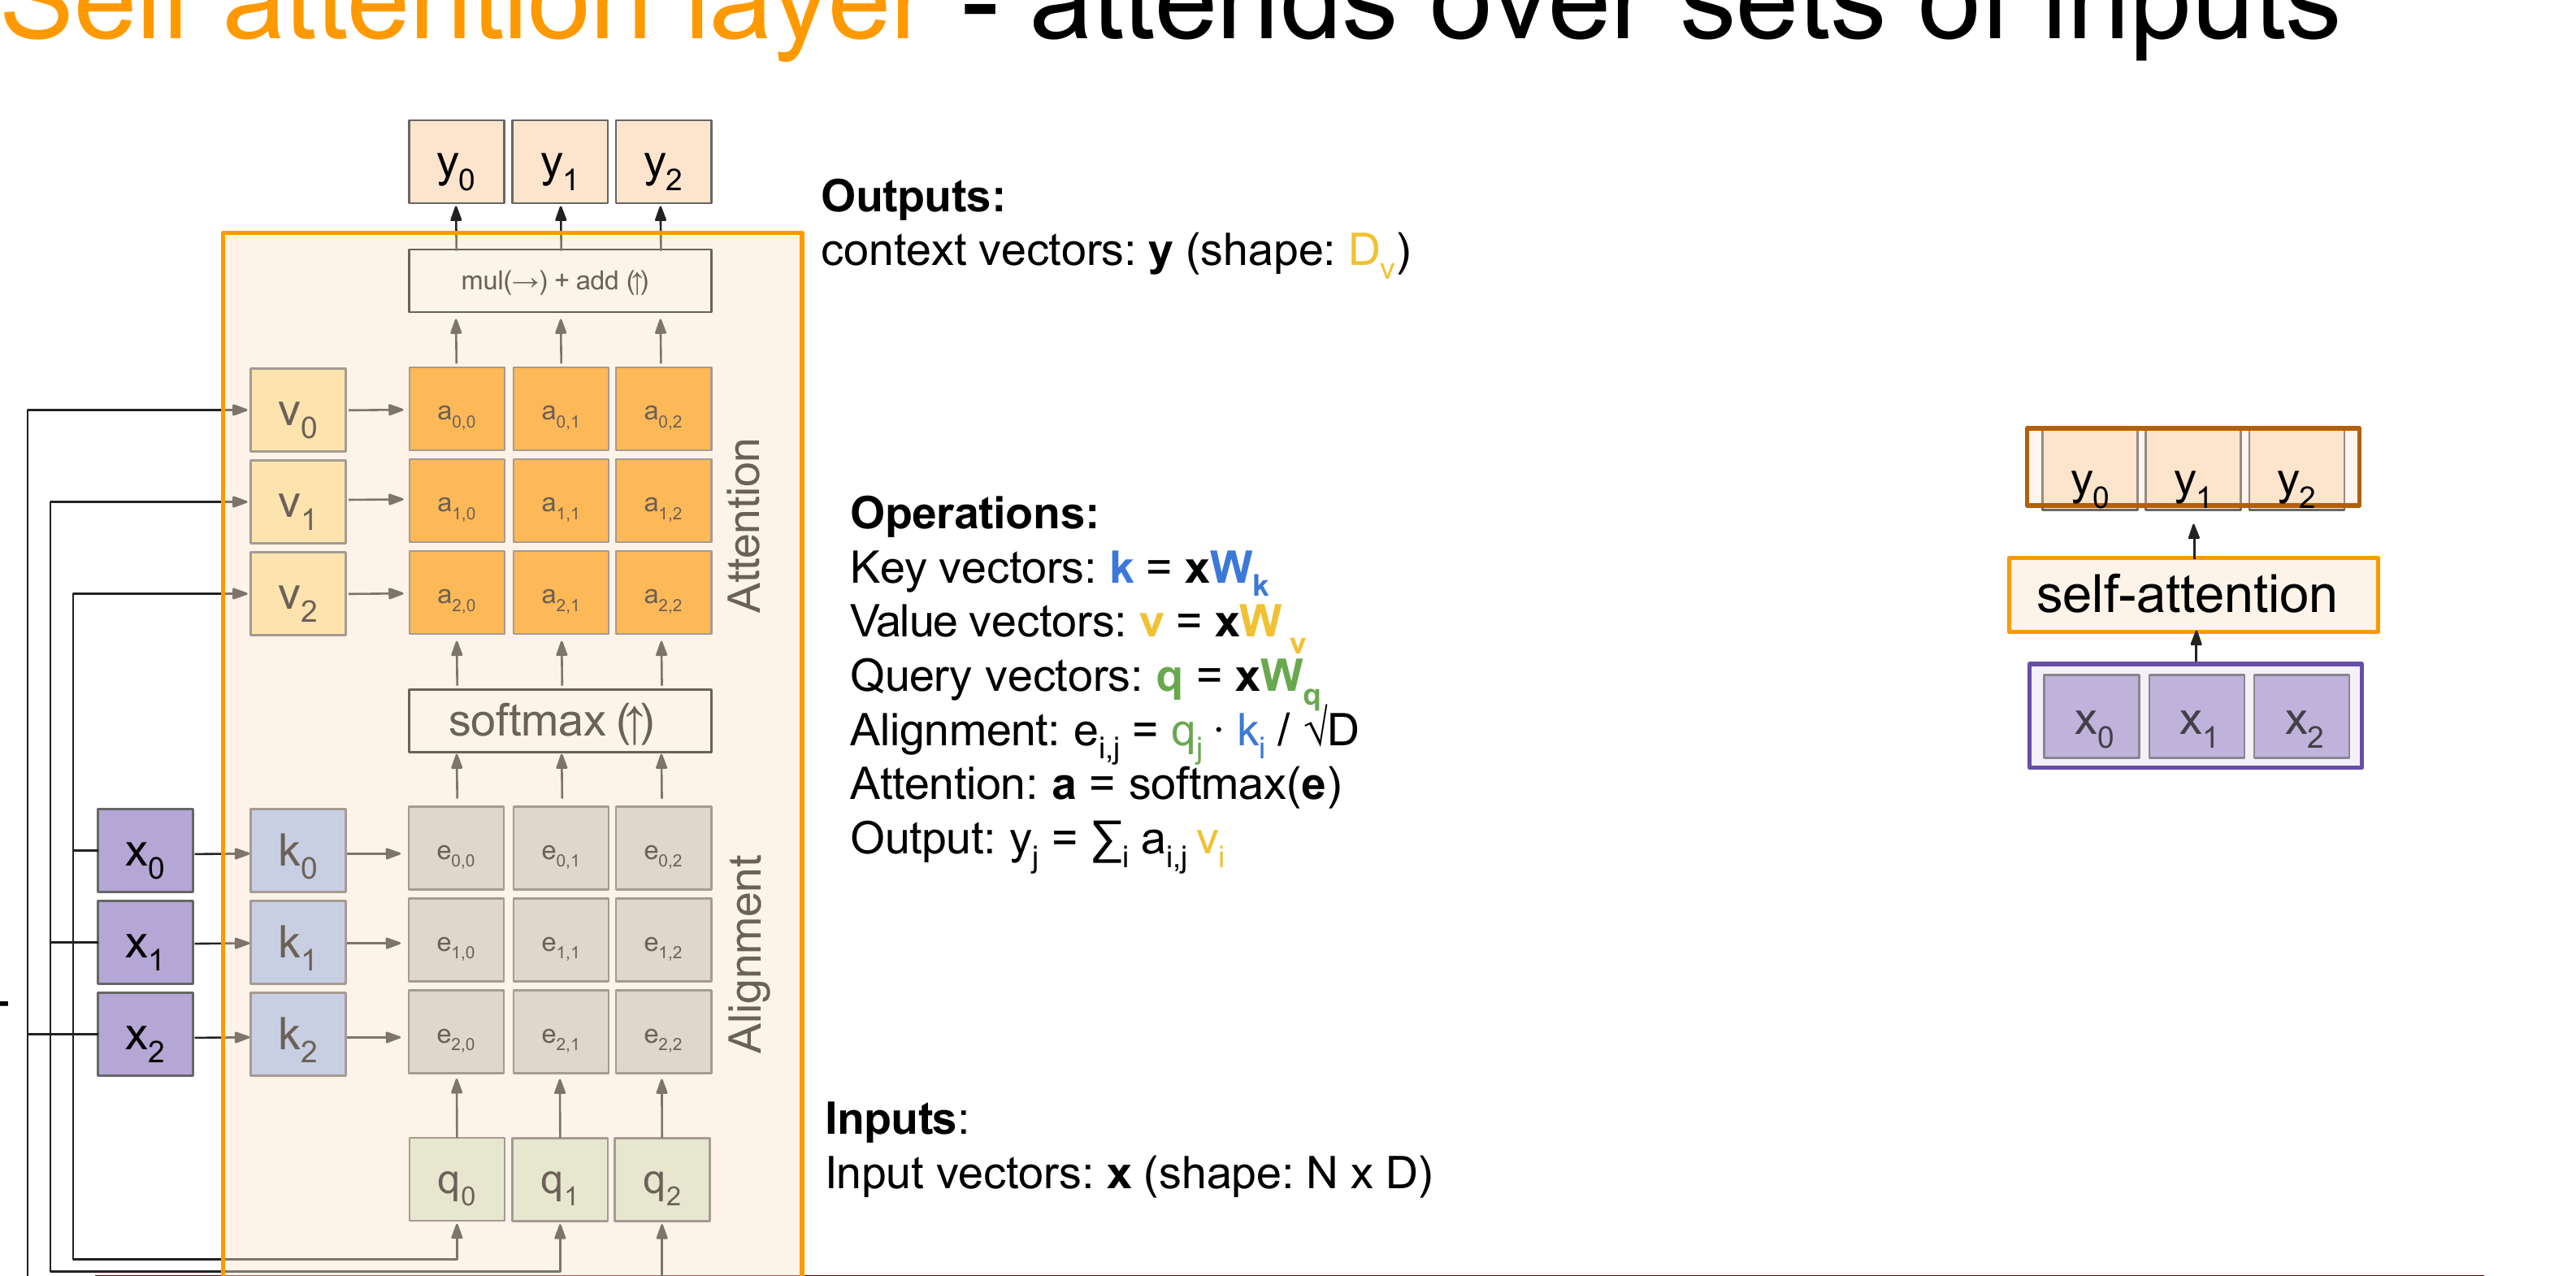
\includegraphics[width=0.92\textwidth]{Pictures/self_attention_layer.png}
    \caption{The Self-Attention layer structure (from course slides). Input vectors are projected into Queries, Keys, and Values. Alignment scores are scaled, normalized via Softmax, and multiplied by Value vectors to produce updated context vectors.}\label{fig:self_attention_layer}
\end{figure}

\subsection{The Query, Key, Value (\texorpdfstring{$Q, K, V$}{Q, K, V}) Formulation}

Given an input matrix $X \in \mathbb{R}^{N \times D}$ representing $N$ tokens of dimension $D$, the self-attention layer linearly projects each vector into three distinct roles through learnable parameter matrices:

\begin{itemize}[leftmargin=*]
    \item \textbf{Query ($Q = X W_Q \in \mathbb{R}^{N \times D_k}$):} Represents what the current token is looking for.
    \item \textbf{Key ($K = X W_K \in \mathbb{R}^{N \times D_k}$):} Represents the identity or content descriptor against which queries are compared.
    \item \textbf{Value ($V = X W_V \in \mathbb{R}^{N \times D_v}$):} The actual informational content retrieved and blended into the updated representation.
\end{itemize}

The pairwise alignment score between token $j$ (query) and token $i$ (key) is evaluated via their dot product, scaled by the square root of the key dimension $D_k$:
\begin{equation}
    e_{i, j} = \frac{q_j^T k_i}{\sqrt{D_k}}
\end{equation}
In compact matrix notation, the \textbf{Scaled Dot-Product Attention} introduced by Vaswani et al.~\cite{vaswani2017attention} is evaluated simultaneously across all tokens:
\begin{equation}
    \operatorname{Attention}(Q, K, V) = \operatorname{softmax}\left(\frac{Q K^T}{\sqrt{D_k}}\right) V
    \label{eq:scaled_dot_product}
\end{equation}

\begin{Notebox}
\textbf{Why Divide by $\sqrt{D_k}$?} \\
Assume the components of query $q$ and key $k$ are independent random variables with zero mean and unit variance. Their dot product $q^T k = \sum_{m=1}^{D_k} q_m k_m$ has mean $0$ and variance $D_k$. 

For large dimensions (e.g., $D_k = 64$ or $D_k = 128$), the variance of the dot products becomes substantial ($D_k \gg 1$), resulting in large positive or negative logits. Passing large inputs into Softmax forces its outputs to saturate near $0$ or $1$, causing the local gradient of Softmax to collapse exponentially toward zero. Dividing by $\sqrt{D_k}$ normalizes the variance back to $1$, preserving healthy gradient flow throughout training.
\end{Notebox}

\subsection{Maximum Path Length and Computational Complexity}

The structural dominance of self-attention over recurrent and convolutional layers stems from its \textbf{constant path length} and \textbf{unconstrained parallelizability}, illustrated in Figure~\ref{fig:path_length_comparison}.

\begin{figure}[htbp]
    \centering
    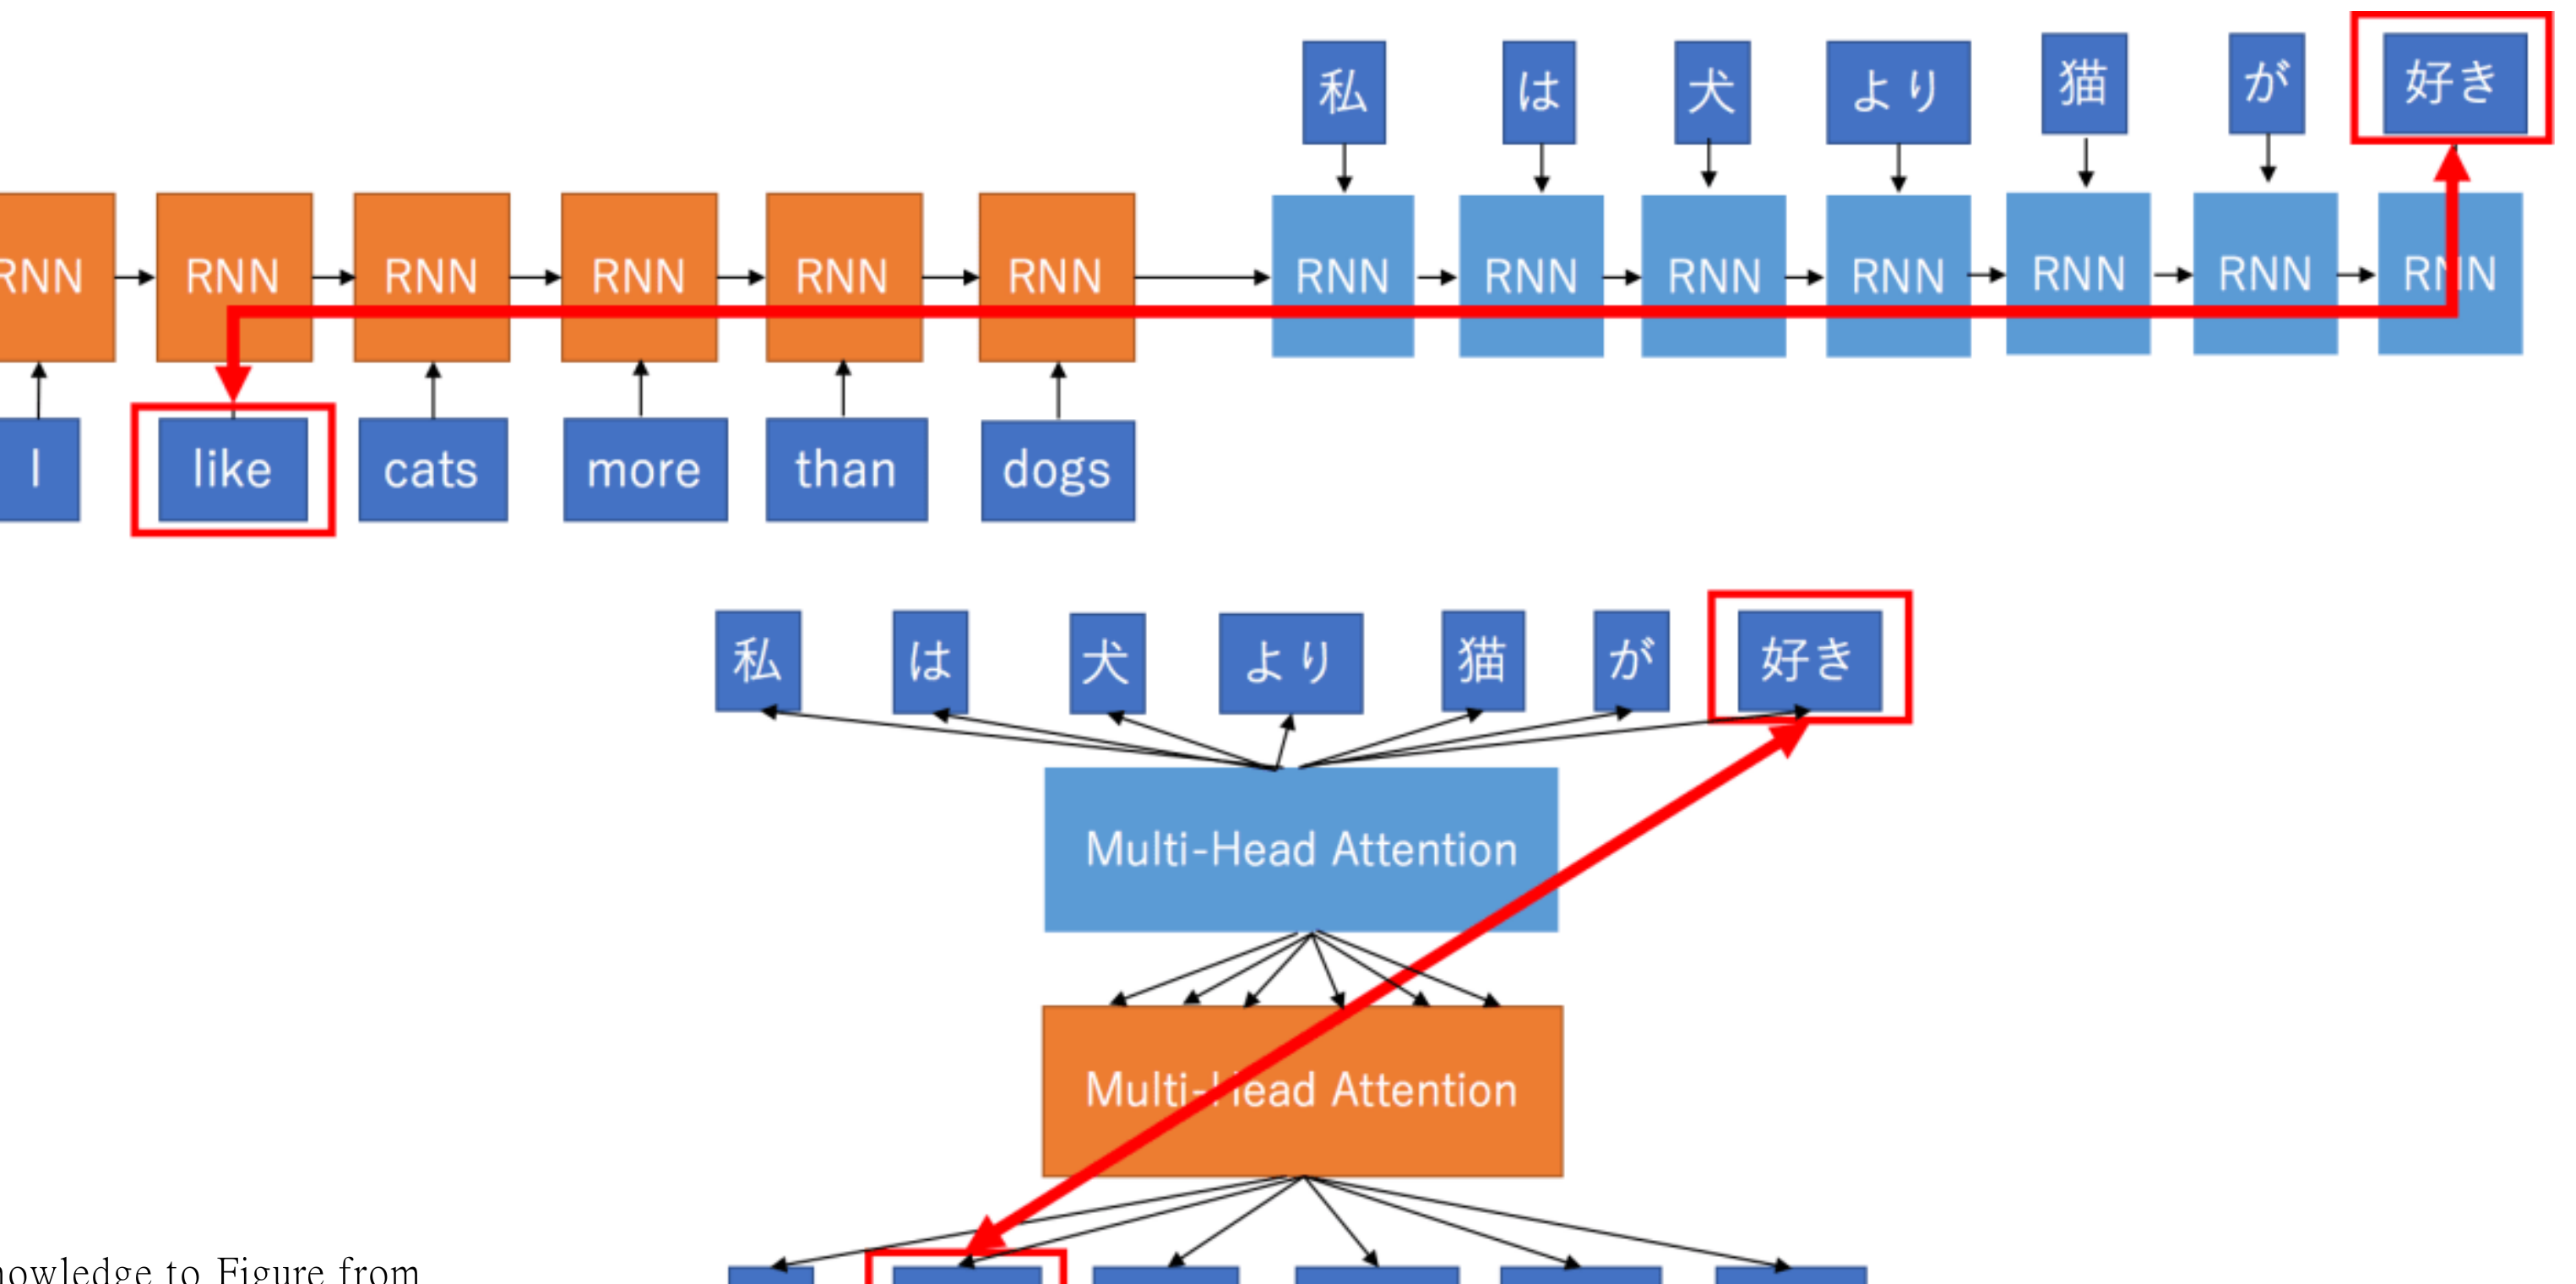
\includegraphics[width=0.88\textwidth]{Pictures/path_length_comparison.png}
    \caption{Maximum path length comparison between RNN and Self-Attention (from course slides). In an RNN, connecting position $1$ to position $n$ requires $O(n)$ sequential hops. In Self-Attention, any pair of tokens communicates directly in a single $O(1)$ constant step.}\label{fig:path_length_comparison}
\end{figure}

Table~\ref{tab:layer_comparison} synthesizes the asymptotic properties from course Slide 45 (Vaswani et al.~\cite{vaswani2017attention}):

\begin{table}[htbp]
\centering
\small
\renewcommand{\arraystretch}{1.2}
\begin{tabular}{l c c c}
\toprule
\textbf{Layer Type} & \textbf{Complexity per Layer} & \textbf{Sequential Operations} & \textbf{Maximum Path Length} \\
\midrule
\textbf{Self-Attention} & $O(n^2 \cdot d)$ & $O(1)$ & $O(1)$ \\
\textbf{Recurrent (RNN/LSTM)} & $O(n \cdot d^2)$ & $O(n)$ & $O(n)$ \\
\textbf{Convolutional} & $O(k \cdot n \cdot d^2)$ & $O(1)$ & $O(\log_k(n))$ \\
\bottomrule
\end{tabular}
\caption{Comparative analysis of Self-Attention, Recurrence, and Convolutions.}\label{tab:layer_comparison}
\end{table}

\begin{itemize}[leftmargin=*]
    \item \textbf{Sequential Operations ($O(1)$ vs $O(n)$):} While an RNN must evaluate $n$ sequential steps to process $n$ tokens, Self-Attention computes all $n \times n$ attention scores in parallel via matrix multiplications.
    \item \textbf{Maximum Path Length ($O(1)$ vs $O(n)$):} The shortest path that gradient signals must travel between any two arbitrary positions is strictly $1$. There is no intermediate chain of recurrent weights, eliminating structural vanishing gradients across long temporal horizons.
    \item \textbf{Memory Scalability Trade-off ($O(n^2 \cdot d)$):} Because self-attention computes an $n \times n$ attention matrix, memory consumption grows quadratically with sequence length $n$. While efficient when $n < d$ (e.g., $n = 512, d = 1024$), ultra-long sequences require specialized sparse or linear attention formulations.
\end{itemize}


\section{Positional Encodings, Masking, and Multi-Head Attention}

\subsection{Permutation Equivariance: Why Pure Attention Ignores Order}

A fundamental property of the self-attention formula (Equation~\ref{eq:scaled_dot_product}) is that it is \textbf{permutation equivariant}:
\begin{equation}
    \operatorname{Attention}(P Q, P K, P V) = P \operatorname{Attention}(Q, K, V)
\end{equation}
for any permutation matrix $P$. If we shuffle the order of the input tokens, the output tokens are shuffled in the exact same manner without changing their computed values. Because natural language and physical signals depend critically on temporal or spatial order, pure self-attention requires an explicit mechanism to inject positional awareness.

\subsection{Positional Encodings (PE)}

To convey token order, a positional vector $p_j \in \mathbb{R}^D$ is added directly to each input embedding $x_j$:
\begin{equation}
    \widetilde{x}_j = x_j + p_j
\end{equation}
Course Slide 50 formalizes the four core desiderata for any positional encoding function $\operatorname{pos}(j)$:
\begin{enumerate}[nosep, leftmargin=*]
    \item It must output a unique encoding for each time step $j$.
    \item The geometric distance between any two time steps $(j, j+k)$ must remain consistent across sentences of varying lengths.
    \item It must generalize effortlessly to longer sequence lengths at test time, producing bounded activation values.
    \item It must be deterministic.
\end{enumerate}

\begin{figure}[htbp]
    \centering
    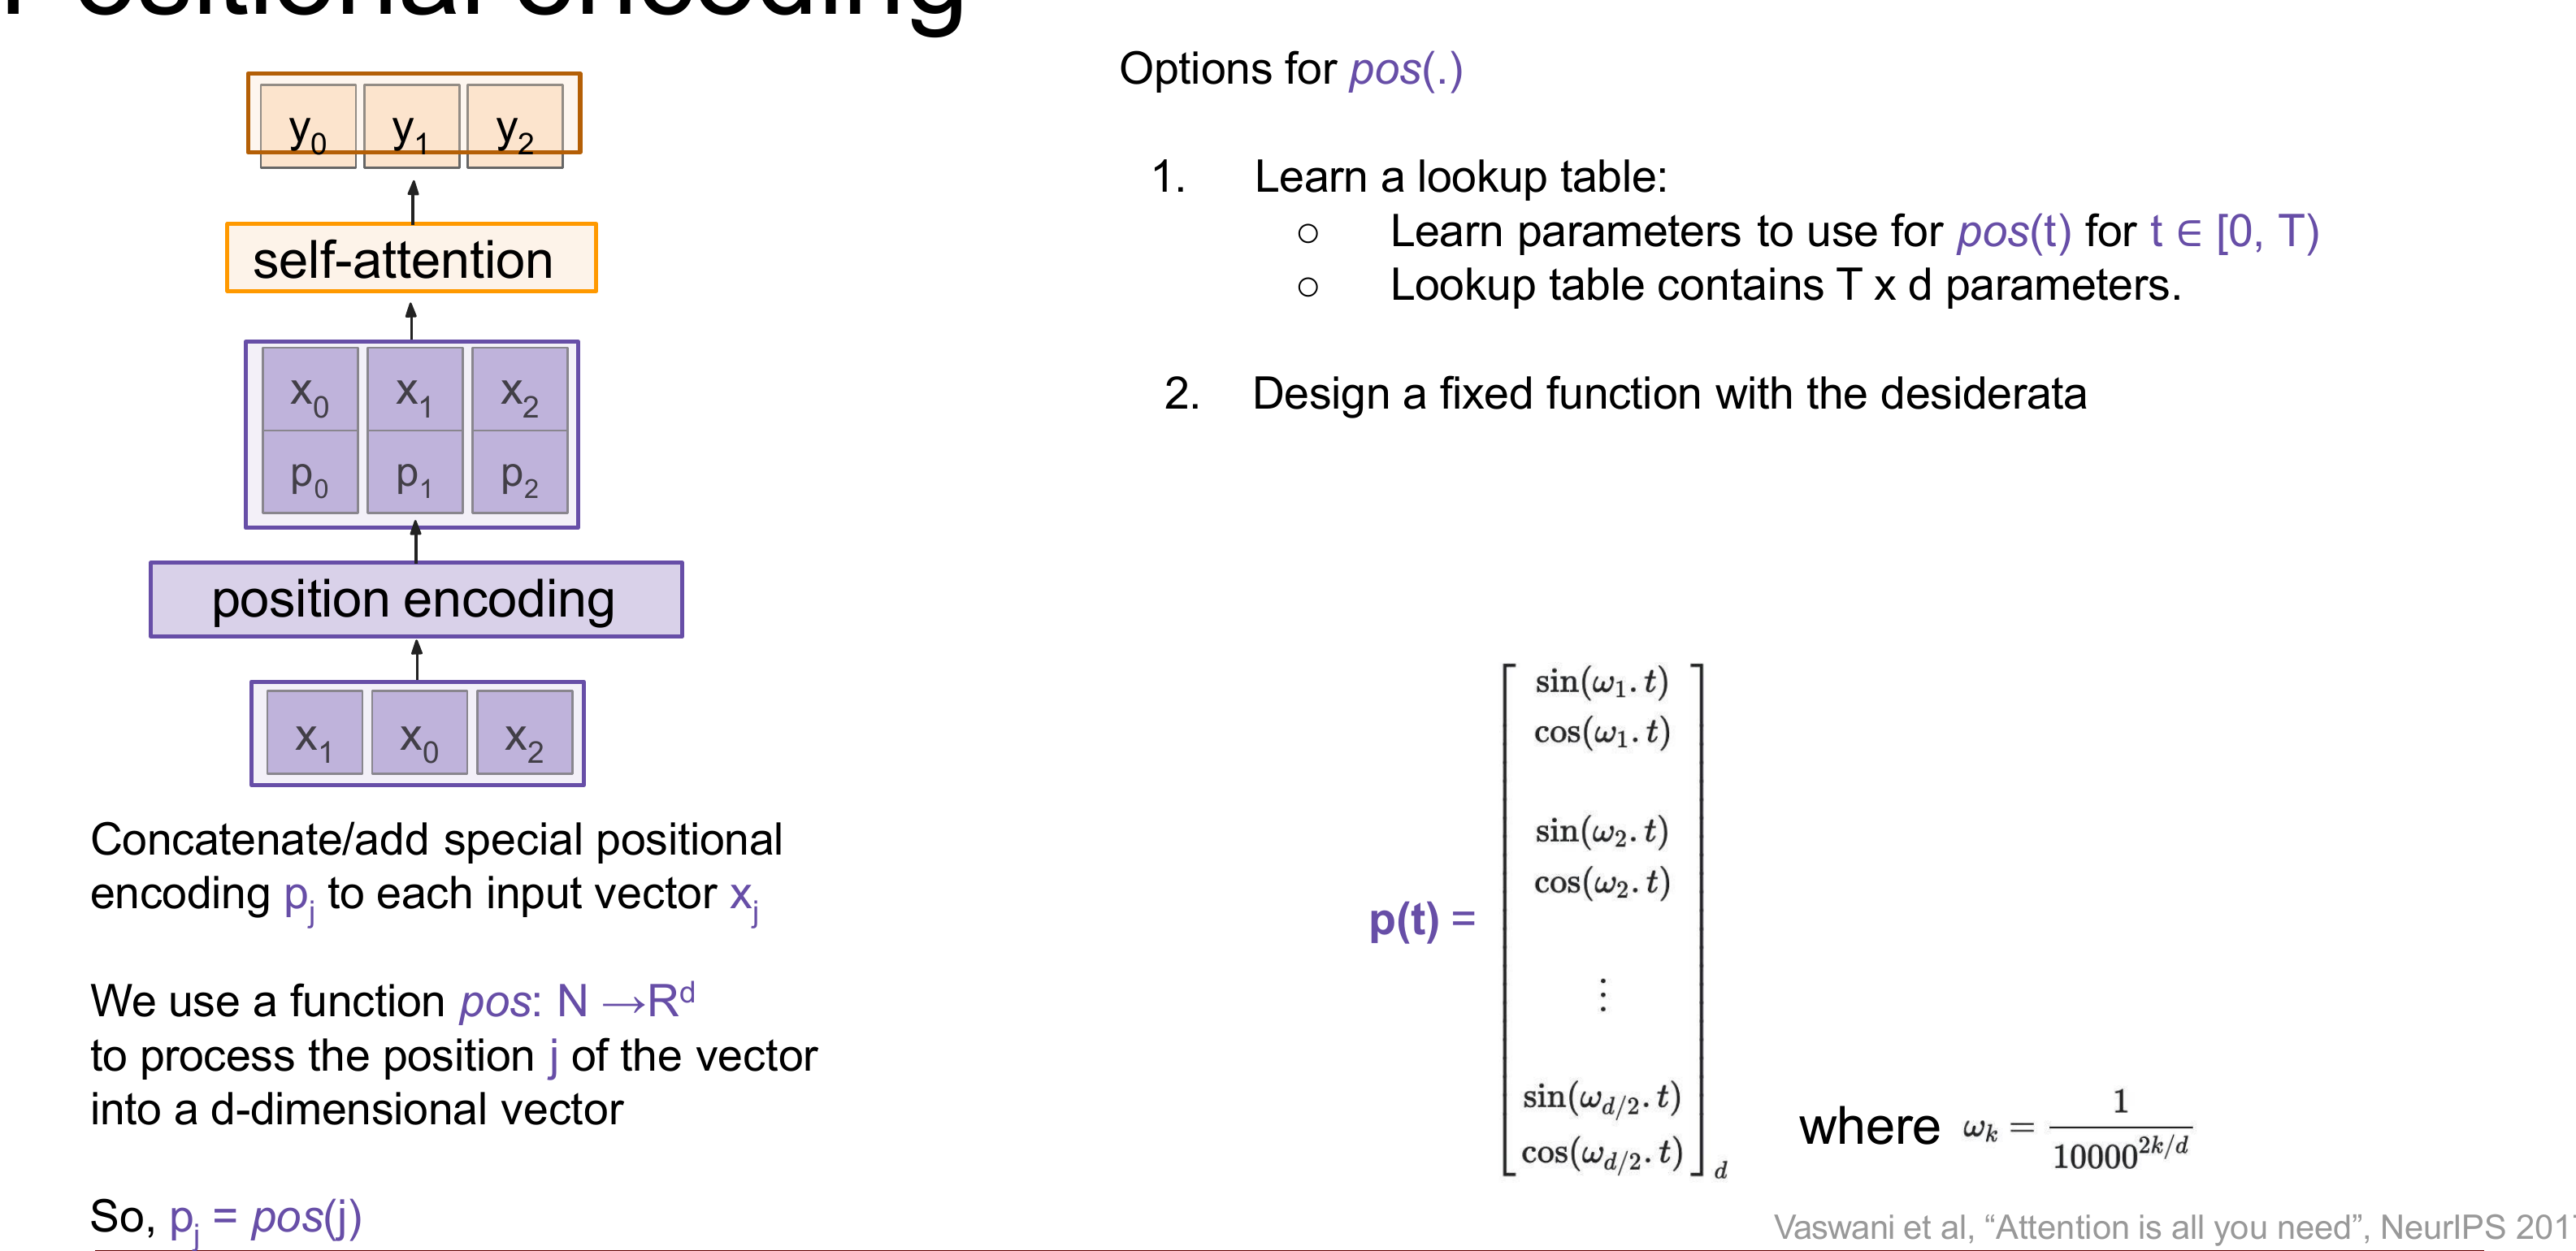
\includegraphics[width=0.88\textwidth]{Pictures/positional_encoding_waves.png}
    \caption{Sinusoidal Positional Encoding (Vaswani et al.~\cite{vaswani2017attention}, from course slides). Each position $t$ is mapped to a combination of sinusoidal waves across frequencies, allowing the model to attend by relative distances.}\label{fig:positional_encoding_waves}
\end{figure}

Two primary paradigms exist for generating $p_j$:
\begin{itemize}[leftmargin=*]
    \item \textbf{Learned Positional Embeddings:} A trainable lookup table of shape $(T_{\text{max}} \times D)$ is optimized alongside model parameters. While flexible, it cannot generalize beyond the maximum sequence length $T_{\text{max}}$ observed during training.
    \item \textbf{Sinusoidal Positional Encoding (Vaswani et al.~\cite{vaswani2017attention}):} Pre-computed using sine and cosine functions of varying frequencies, illustrated in Figure~\ref{fig:positional_encoding_waves}:
    \begin{align}
        PE_{(pos, 2i)} &= \sin\left(\frac{pos}{10000^{2i/D}}\right) \\
        PE_{(pos, 2i+1)} &= \cos\left(\frac{pos}{10000^{2i/D}}\right)
    \end{align}
    where $pos$ is the token position and $i \in \{0, \dots, D/2 - 1\}$ indexes the channel dimension.
\end{itemize}

\begin{keywordbox}
\textbf{The Linear Relative Transformation Property} \\
Because $\sin(\alpha + \beta) = \sin\alpha\cos\beta + \cos\alpha\sin\beta$ and $\cos(\alpha + \beta) = \cos\alpha\cos\beta - \sin\alpha\sin\beta$, for any fixed offset $k$, the positional encoding at position $pos + k$ can be represented as a linear transformation of the encoding at position $pos$:
\[ PE_{(pos+k)} = M_k \cdot PE_{(pos)} \]
where $M_k \in \mathbb{R}^{D \times D}$ is a deterministic rotation matrix. This allows self-attention to easily learn to attend based on \textbf{relative positional offsets}.
\end{keywordbox}

\subsection{Masked Self-Attention (Causal Attention)}

In autoregressive generation tasks (such as language modeling or autoregressive translation decoding), token $y_t$ must be generated using only past context $y_{<t}$ and must never access future tokens $y_{t+1}, \dots, y_T$.

In an RNN, causality is naturally enforced by sequential step-by-step execution. To preserve causality in the Transformer \textbf{without sacrificing parallel training}, we apply a \textbf{Causal Mask} to the alignment scores, as illustrated in Figure~\ref{fig:masked_self_attention_matrix}.

\begin{figure}[htbp]
    \centering
    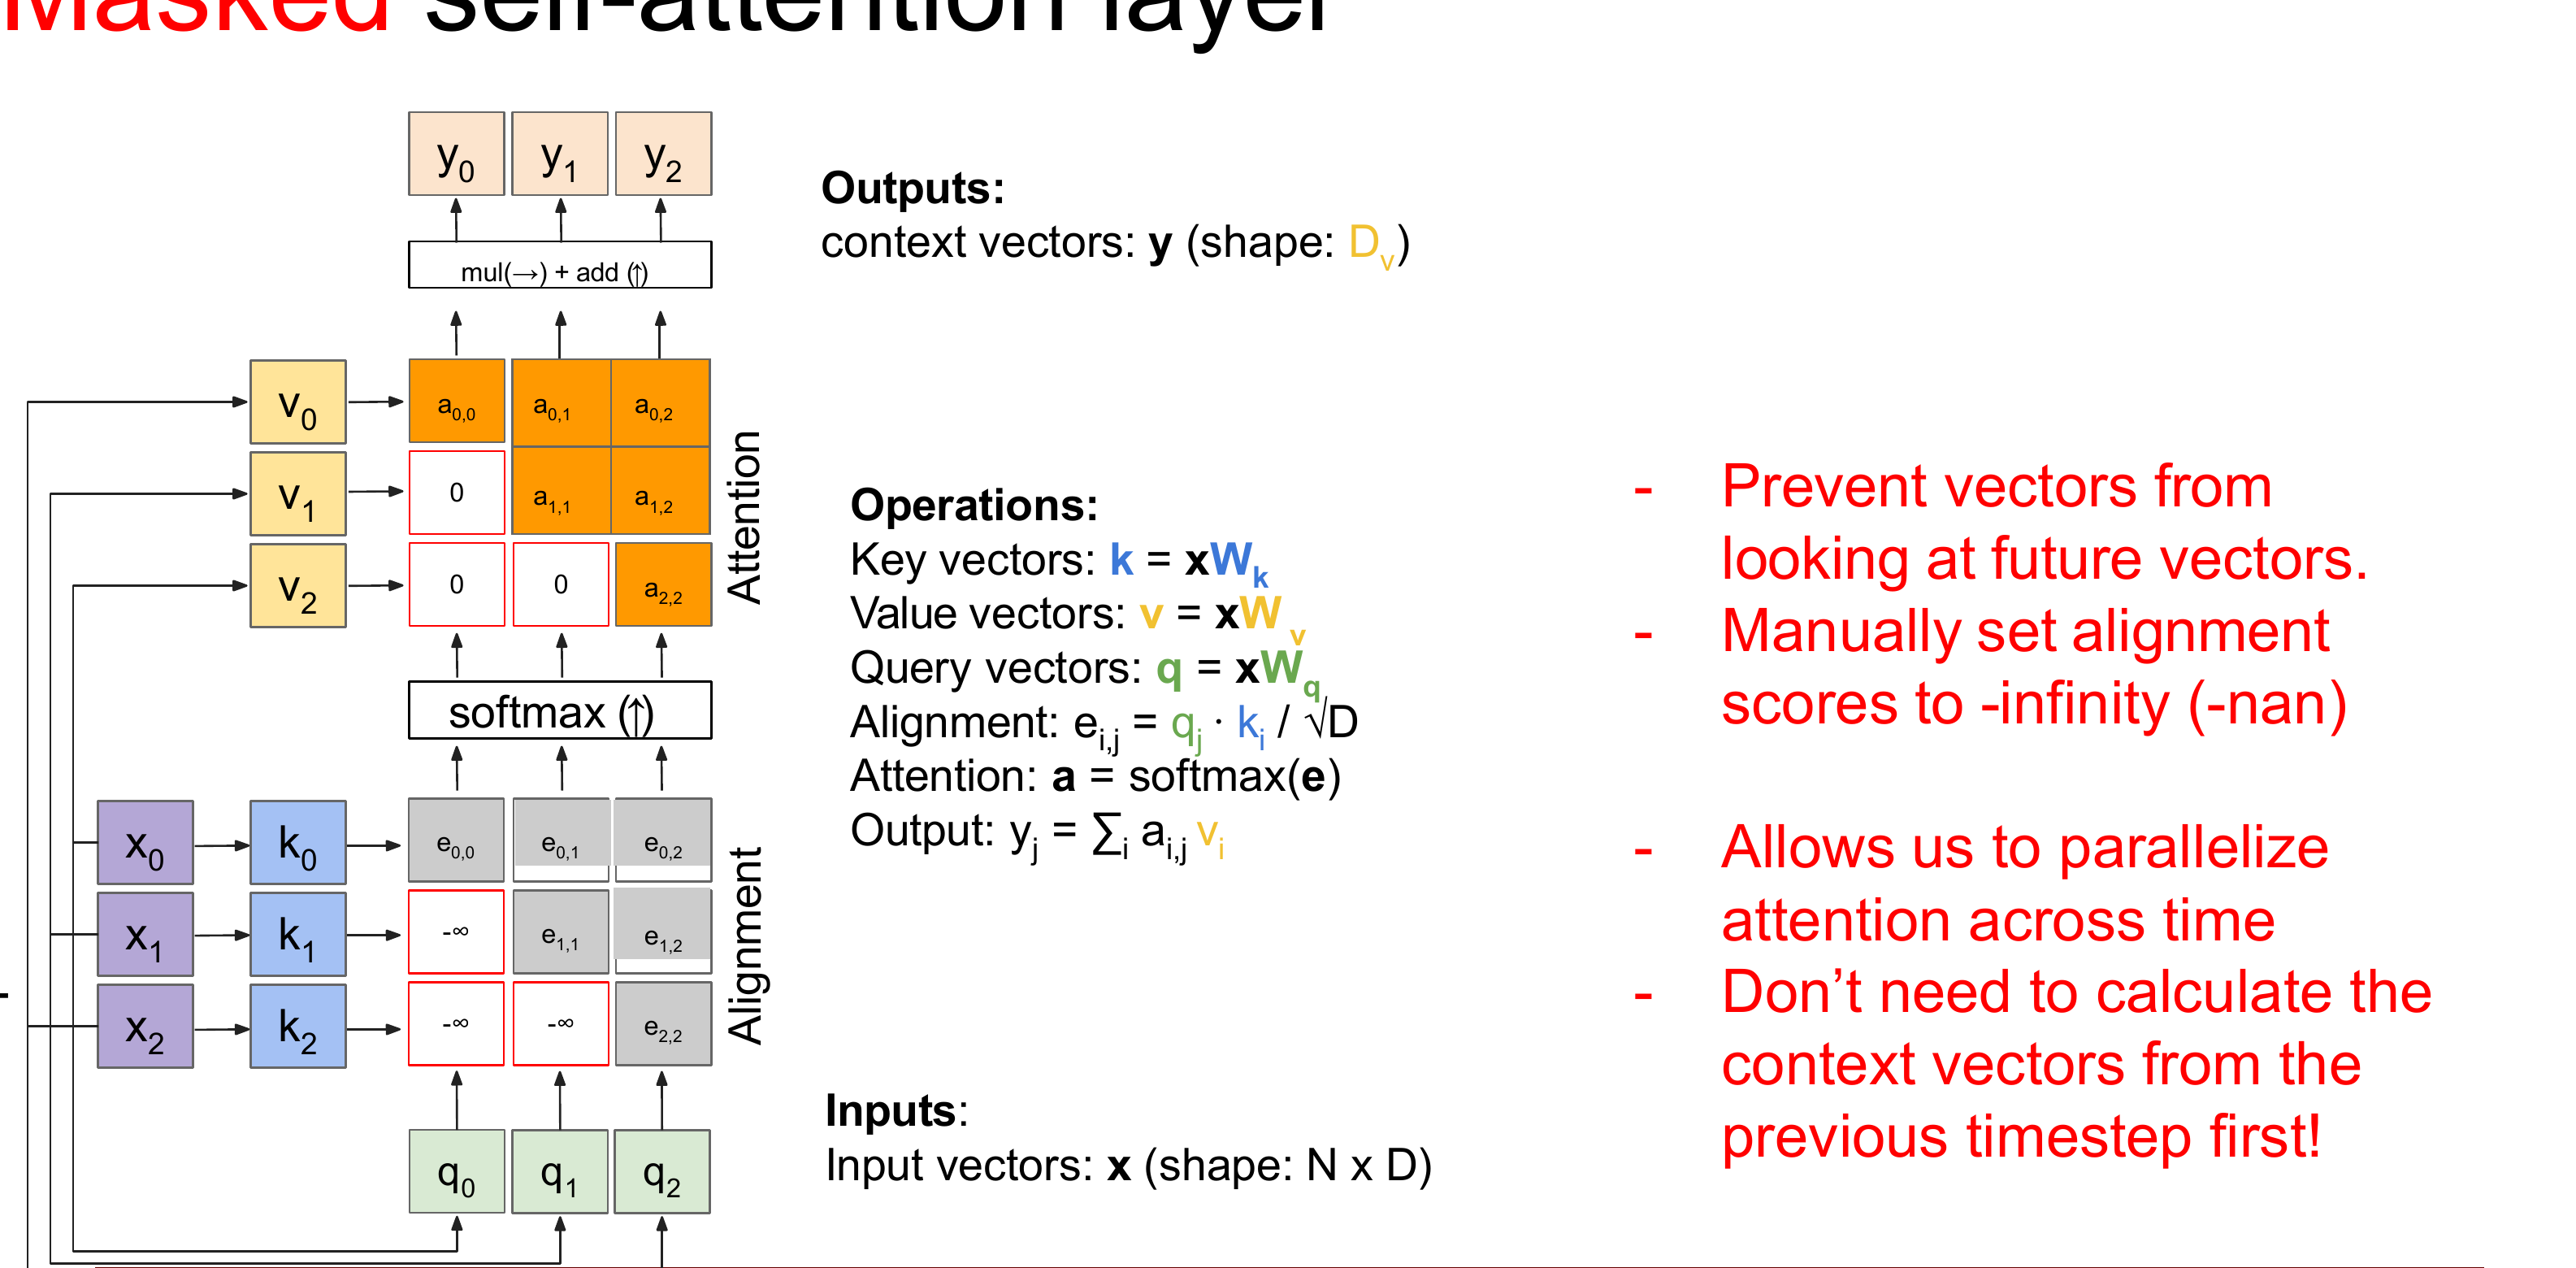
\includegraphics[width=0.88\textwidth]{Pictures/masked_self_attention_matrix.png}
    \caption{Masked Self-Attention with causal masking (from course slides). Setting future alignment entries to $-\infty$ forces their Softmax probabilities to zero, preventing information leakage while enabling full training parallelization across time.}\label{fig:masked_self_attention_matrix}
\end{figure}

Before evaluating the Softmax function, an upper-triangular mask matrix $M$ is added to the scaled dot products:
\begin{equation}
    M_{i, j} = \begin{cases} 0 & \text{if } j \le i \quad \text{(past and current tokens)} \\ -\infty & \text{if } j > i \quad \text{(future tokens)} \end{cases}
\end{equation}
\begin{equation}
    \operatorname{MaskedAttention}(Q, K, V) = \operatorname{softmax}\left(\frac{Q K^T}{\sqrt{D_k}} + M\right) V
\end{equation}
Because $\exp(-\infty) = 0$, the attention weights assigned to future positions evaluate to exactly zero. Consequently, during training, the network can evaluate all $T$ output steps in a single parallel matrix multiplication without unrolling a recurrent loop.

\subsection{Multi-Head Self-Attention (MHSA)}

In single-head attention, computing a single set of attention weights forces the network to average over all relational signals. To provide representational richness, Vaswani et al.~\cite{vaswani2017attention} introduced \textbf{Multi-Head Self-Attention (MHSA)}, shown in Figure~\ref{fig:multihead_attention_layer}.

\begin{figure}[htbp]
    \centering
    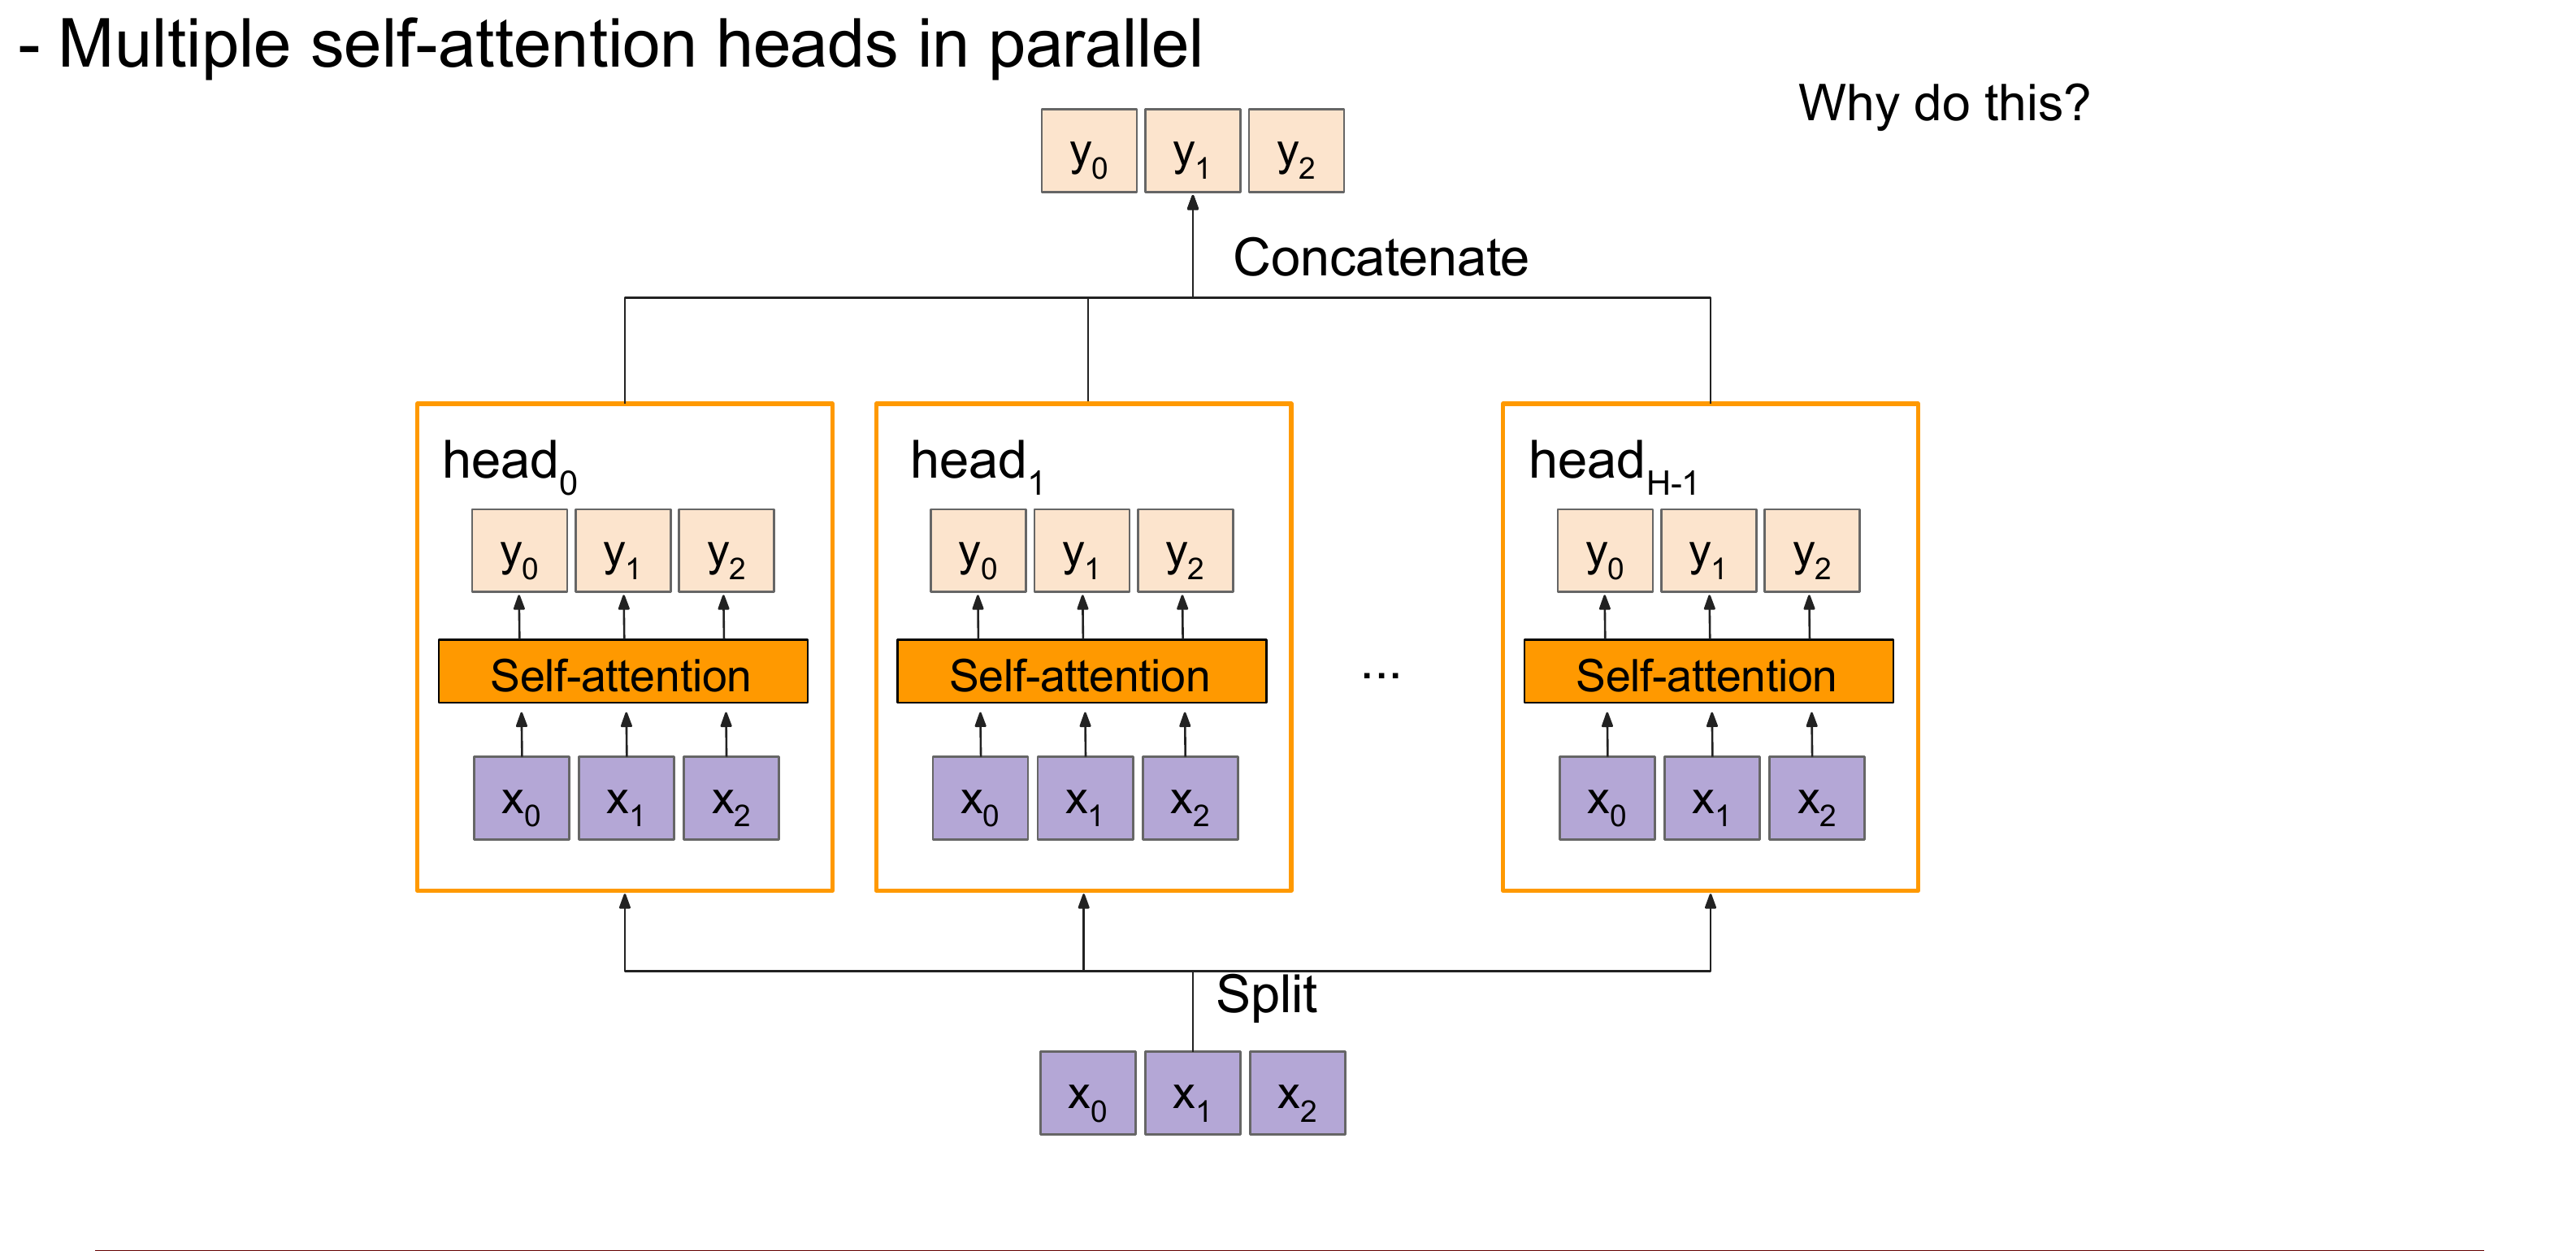
\includegraphics[width=0.88\textwidth]{Pictures/multihead_attention_layer.png}
    \caption{Multi-Head Self-Attention layer (from course slides). Input queries, keys, and values are split across $H$ parallel heads, evaluated independently in separate subspaces, concatenated, and projected through output matrix $W_O$.}\label{fig:multihead_attention_layer}
\end{figure}

\begin{InsightBox}
\textbf{Analogy to Convolutional Filters in CNNs (Slide 59):} \\
In a Convolutional Neural Network, a layer does not learn a single 2D filter; it learns an entire bank of 64 or 128 distinct kernels to simultaneously detect edges, textures, colors, and shapes. 

Multi-Head Attention applies the exact same philosophy to attention: by learning $H$ distinct sets of $(W_i^Q, W_i^K, W_i^V)$ projections, individual heads specialize in distinct relationship patterns (e.g., Head 1 tracks immediate syntactic dependencies, Head 2 tracks pronoun co-reference, and Head 3 tracks long-range semantic topics).
\end{InsightBox}

For $H$ attention heads, the input dimension $D$ is partitioned into head dimension $D_k = D / H$:
\begin{equation}
    \operatorname{head}_i = \operatorname{Attention}\left(Q W_i^Q, \, K W_i^K, \, V W_i^V\right), \quad i \in \{1, \dots, H\}
\end{equation}
where $W_i^Q \in \mathbb{R}^{D \times D_k}$, $W_i^K \in \mathbb{R}^{D \times D_k}$, and $W_i^V \in \mathbb{R}^{D \times D_v}$. The individual outputs are concatenated and linearly projected via output matrix $W_O \in \mathbb{R}^{H D_v \times D}$:
\begin{equation}
    \operatorname{MultiHead}(Q, K, V) = \operatorname{Concat}\left(\operatorname{head}_1, \dots, \operatorname{head}_H\right) W_O
\end{equation}
Because each head operates on vectors of reduced dimension $D / H$, the total computational complexity of MHSA is identical to that of single-head attention on the full dimension $D$.


\section{The Transformer Architecture}

\subsection{The Transformer Encoder Block}

The complete Transformer Encoder is constructed by stacking $N$ identical modular blocks ($N=6$ in the original architecture), detailed in Figure~\ref{fig:transformer_encoder_block}.

\begin{figure}[htbp]
    \centering
    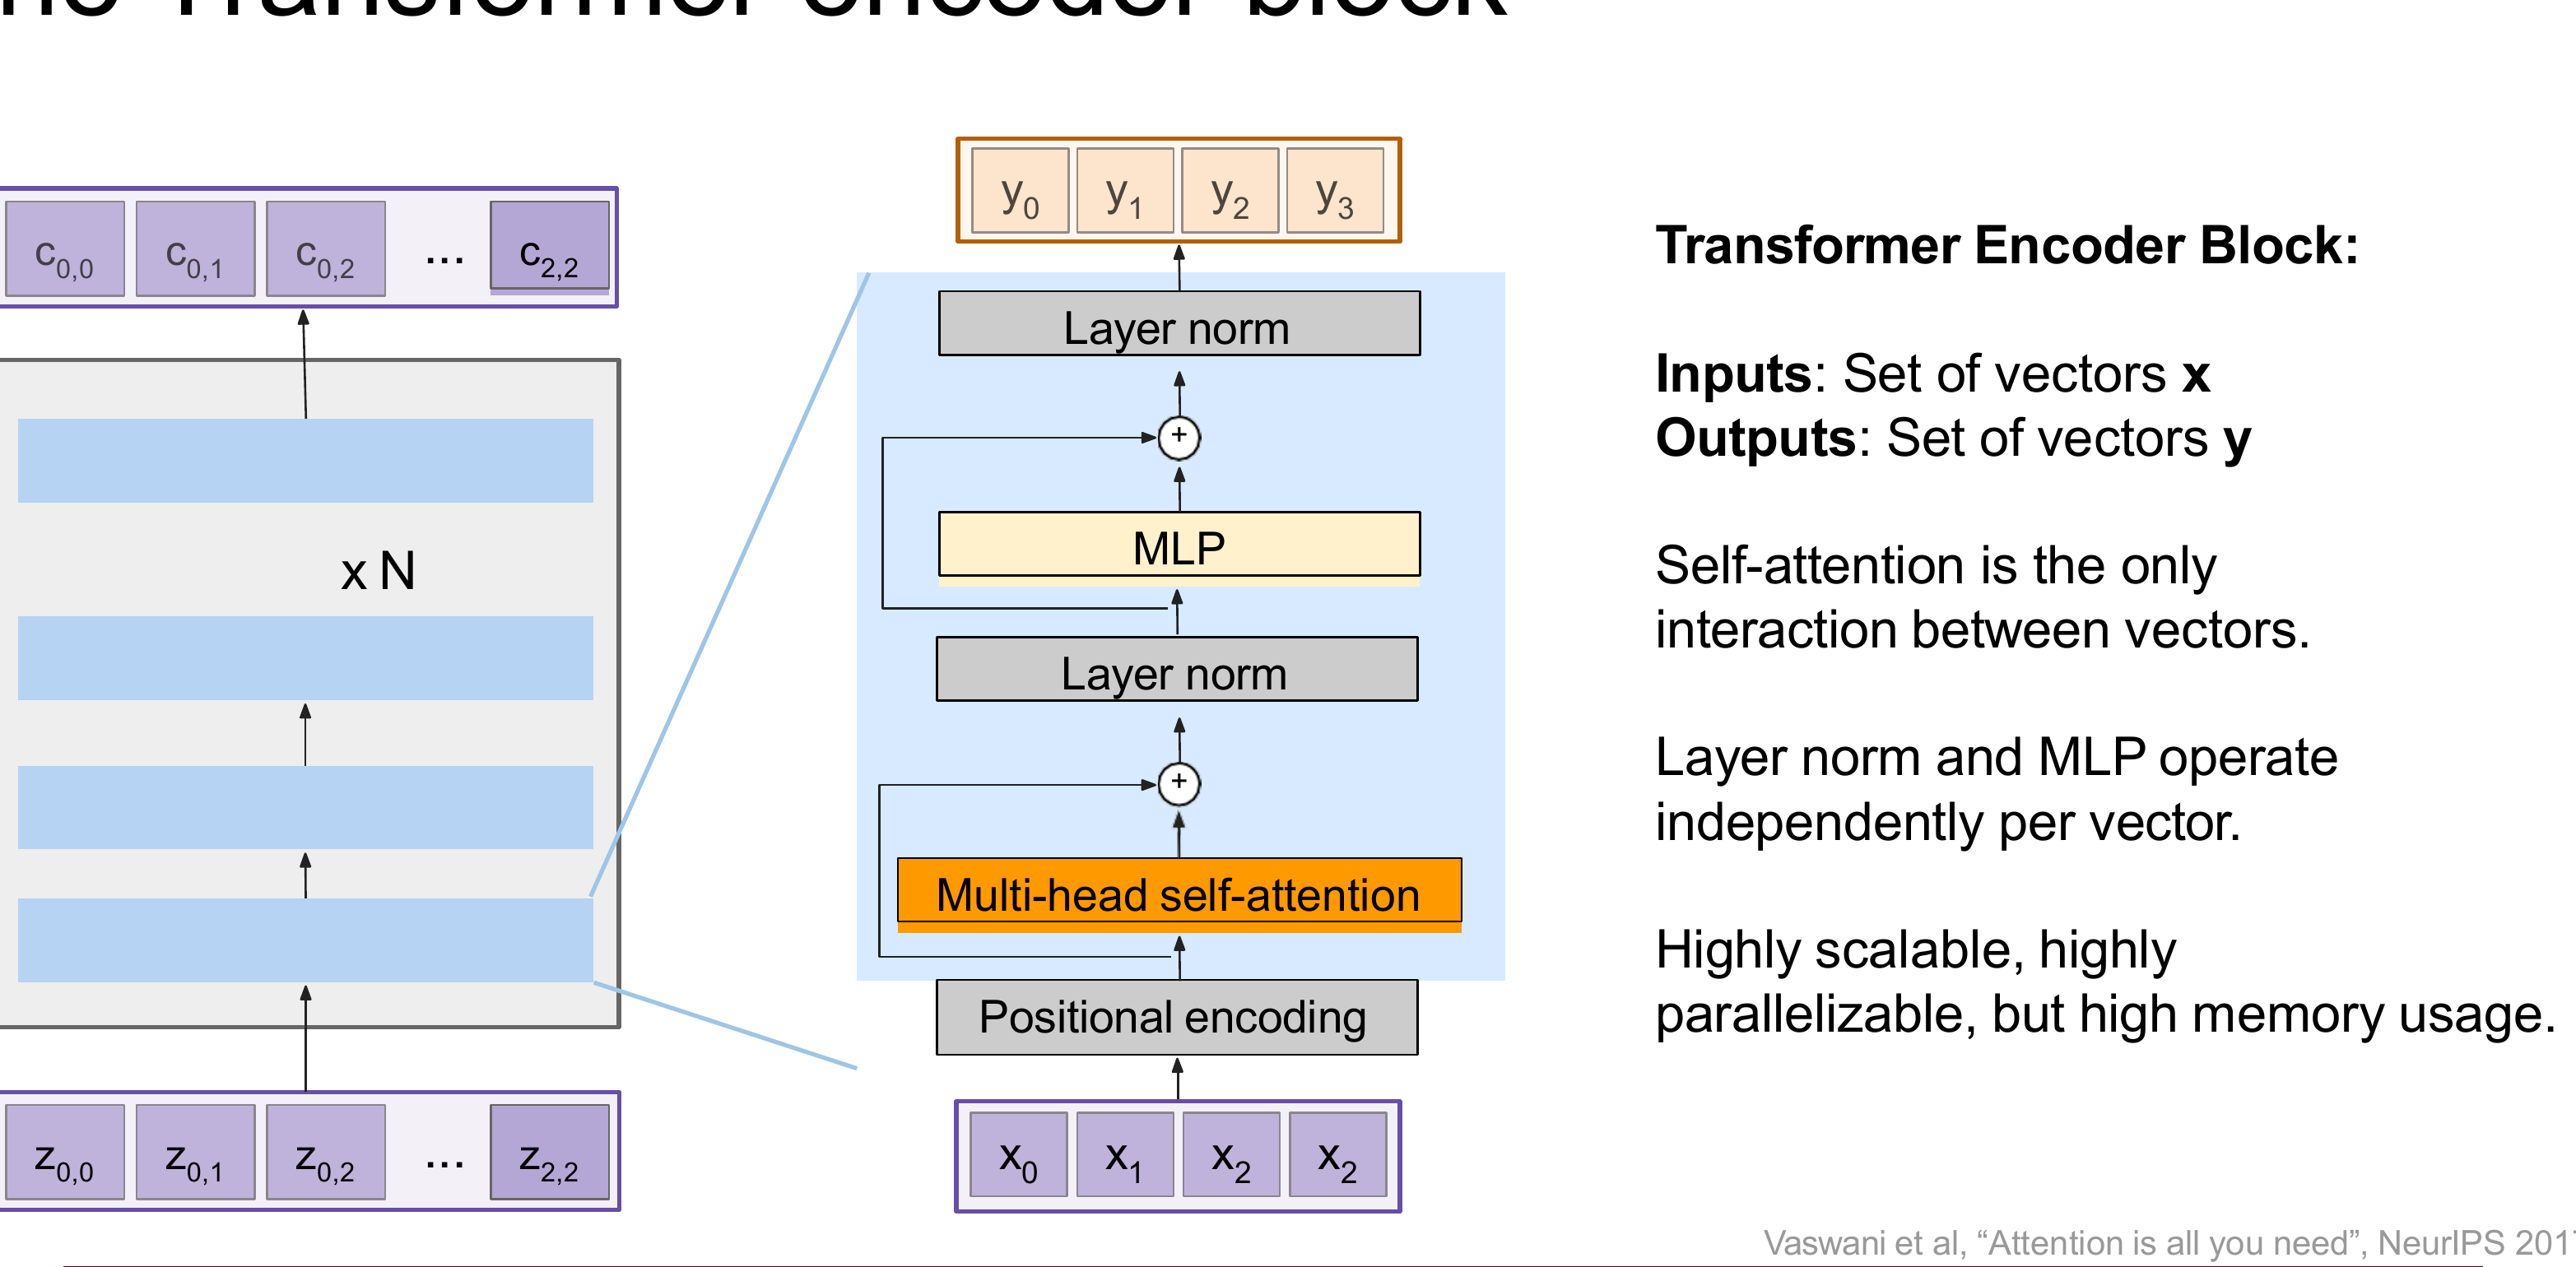
\includegraphics[width=0.72\textwidth]{Pictures/transformer_encoder_block.png}
    \caption{The Transformer Encoder Block (Vaswani et al.~\cite{vaswani2017attention}, from course slides). Composed of Multi-Head Self-Attention followed by a position-wise MLP, each wrapped with residual connections and Layer Normalization.}\label{fig:transformer_encoder_block}
\end{figure}

Each encoder block contains two primary sub-layers:
\begin{enumerate}[leftmargin=*]
    \item \textbf{Sub-layer 1 (Multi-Head Self-Attention):} Computes all-to-all token interactions. Crucially, self-attention is the \textbf{only} component in the encoder where information is exchanged across different tokens.
    \item \textbf{Sub-layer 2 (Position-wise Feed-Forward Network):} An MLP applied identically and independently to each token vector:
    \begin{equation}
        \operatorname{FFN}(x) = \max\left(0, x W_1 + b_1\right) W_2 + b_2
    \end{equation}
    Typically, the inner dimension expands to $4D$ before projecting back to $D$ (e.g., $D = 512 \to 2048 \to 512$).
\end{enumerate}

Every sub-layer is wrapped by a \textbf{Residual Connection} followed by \textbf{Layer Normalization} (Chapter~\ref{ch:foundations}):
\begin{equation}
    x_{\text{out}} = \operatorname{LayerNorm}\left(x + \operatorname{SubLayer}(x)\right)
\end{equation}
Residual connections prevent gradient dissipation across deep stacks, while Layer Normalization stabilizes the activation distributions of individual tokens independently of batch size.

\subsection{The Transformer Decoder Block}

The Transformer Decoder stacks $N$ decoder blocks to generate output sequences autoregressively, detailed in Figure~\ref{fig:transformer_decoder_block}.

\begin{figure}[htbp]
    \centering
    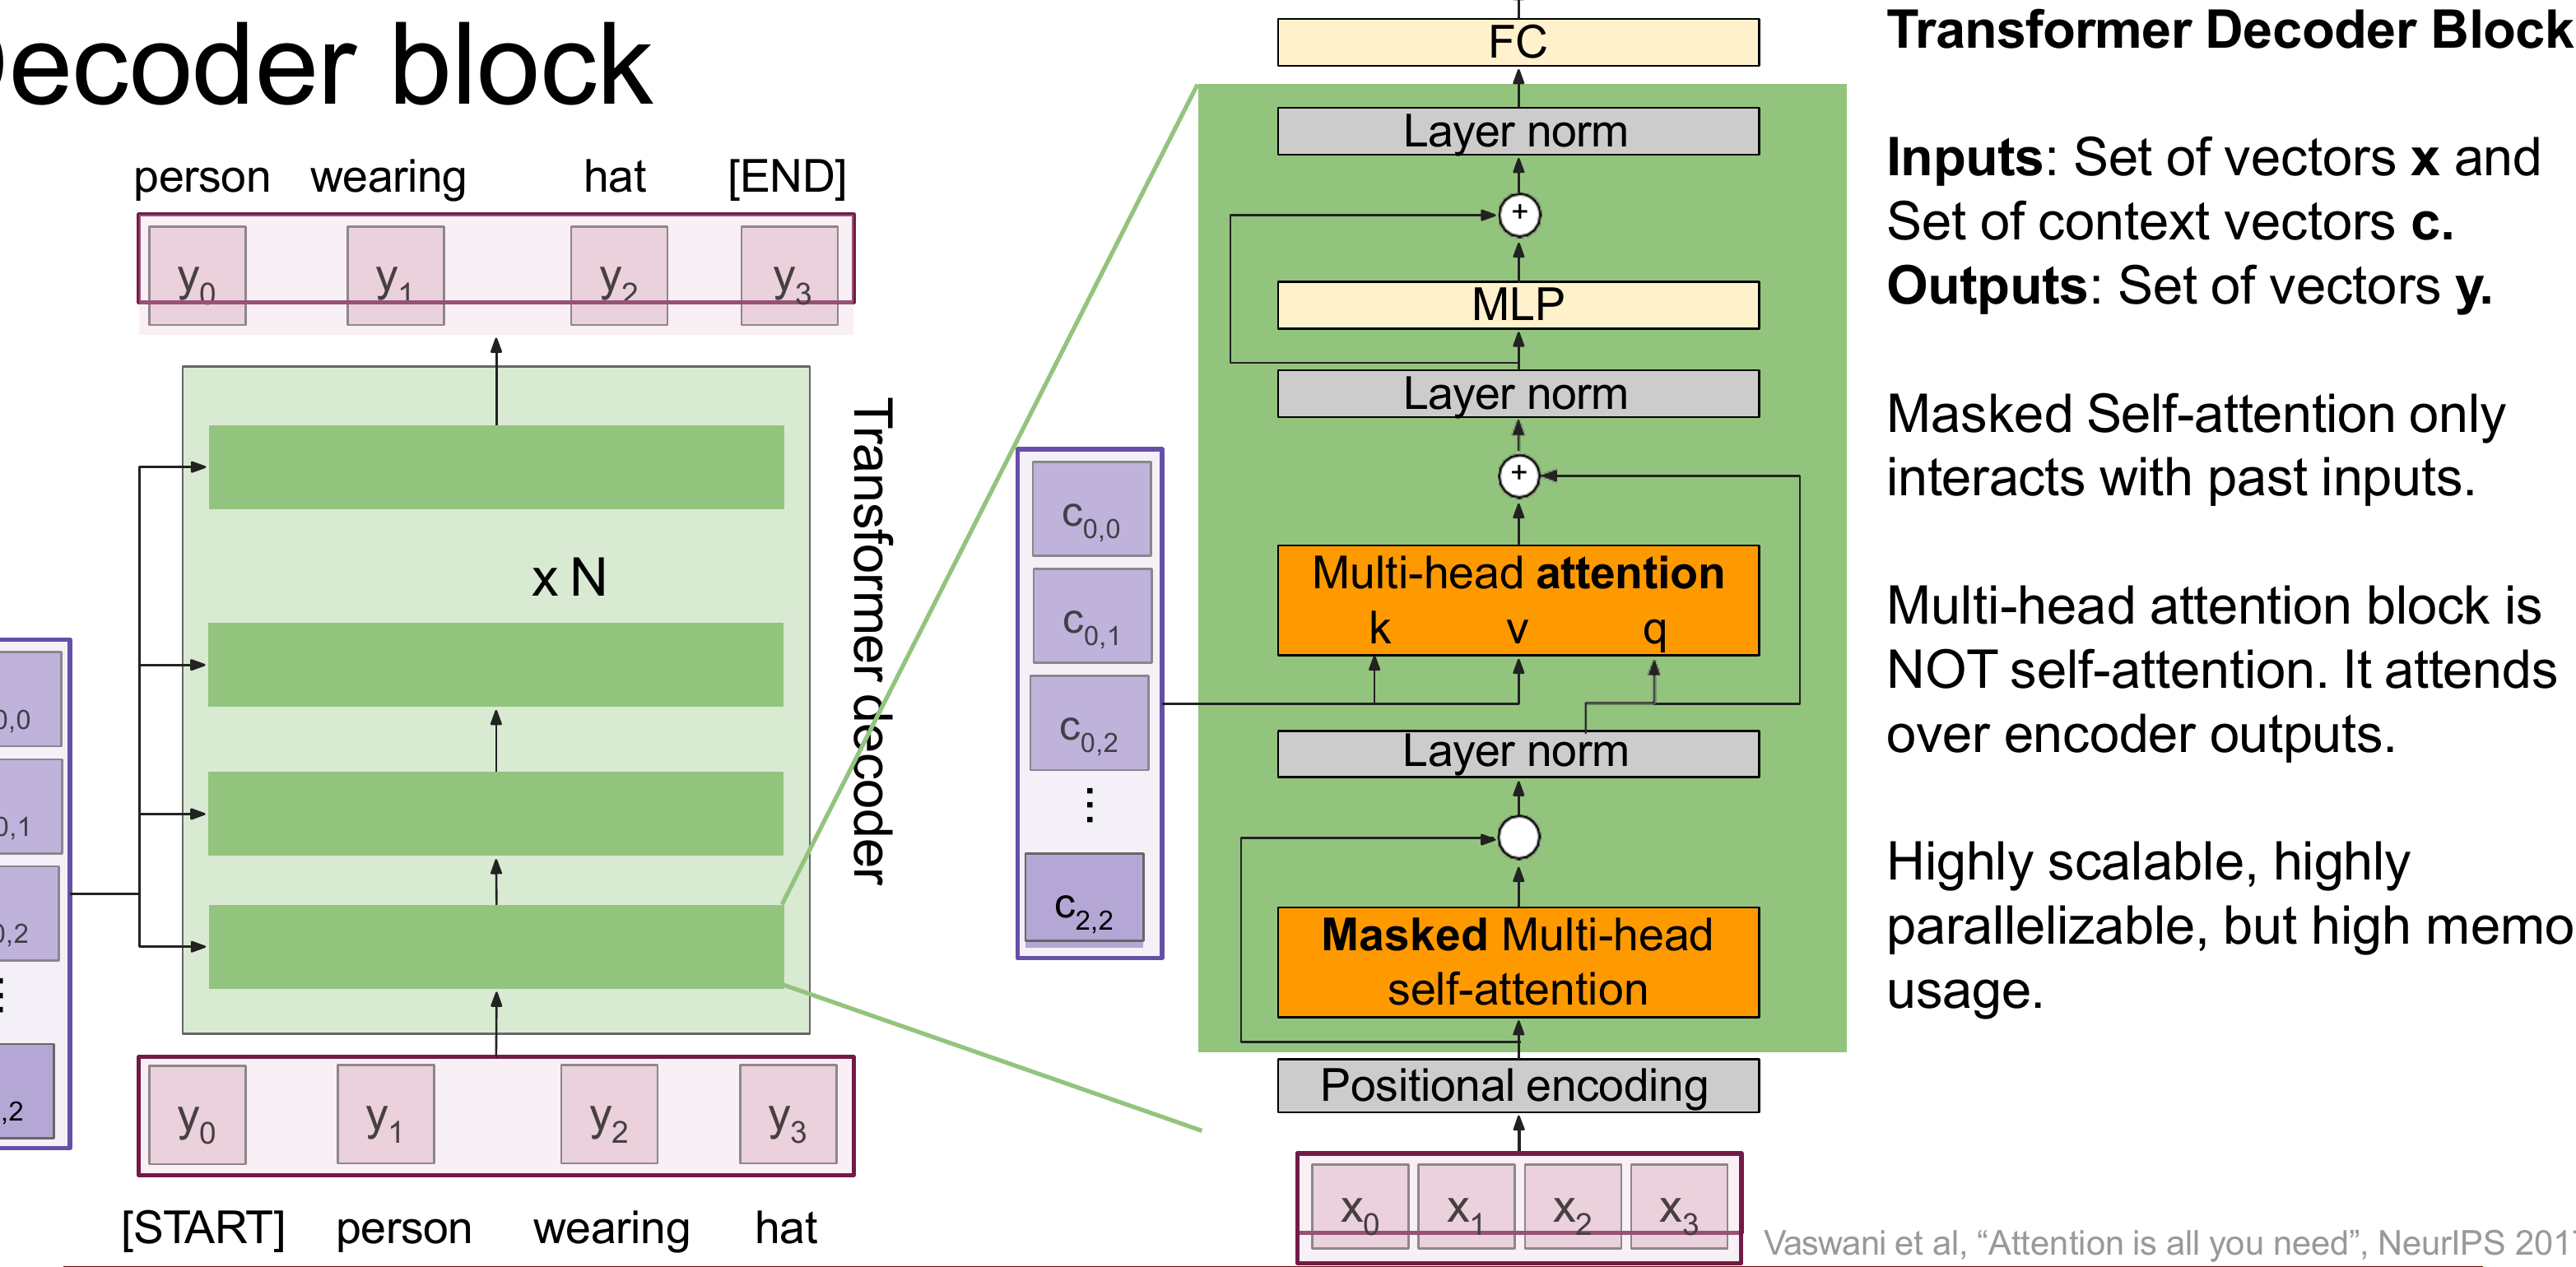
\includegraphics[width=0.72\textwidth]{Pictures/transformer_decoder_block.png}
    \caption{The Transformer Decoder Block (Vaswani et al.~\cite{vaswani2017attention}, from course slides). Contains Masked Multi-Head Self-Attention (causal), Cross-Attention over encoder outputs, and a position-wise MLP.}\label{fig:transformer_decoder_block}
\end{figure}

Each decoder block contains three sub-layers:
\begin{enumerate}[leftmargin=*]
    \item \textbf{Masked Multi-Head Self-Attention:} Computes interactions exclusively among previously generated target tokens using the causal mask ($M_{i,j} = -\infty$ for $j > i$).
    \item \textbf{Multi-Head Cross-Attention:} Fuses encoder and decoder representations. Unlike self-attention, the \textbf{Queries ($Q$)} originate from the preceding decoder layer, while the \textbf{Keys ($K$)} and \textbf{Values ($V$)} are drawn from the final output of the Encoder stack $c$.
    \item \textbf{Position-wise Feed-Forward Network (MLP):} Projects each token vector independently, followed by a final linear classifier and Softmax over the target vocabulary.
\end{enumerate}

\subsection{Comparative Summary: RNNs versus Transformers}

Course Slide 71 provides a side-by-side synthesis of the two paradigms, summarized in Figure~\ref{fig:rnn_vs_transformer_table} and Table~\ref{tab:rnn_vs_transformer}.

\begin{figure}[htbp]
    \centering
    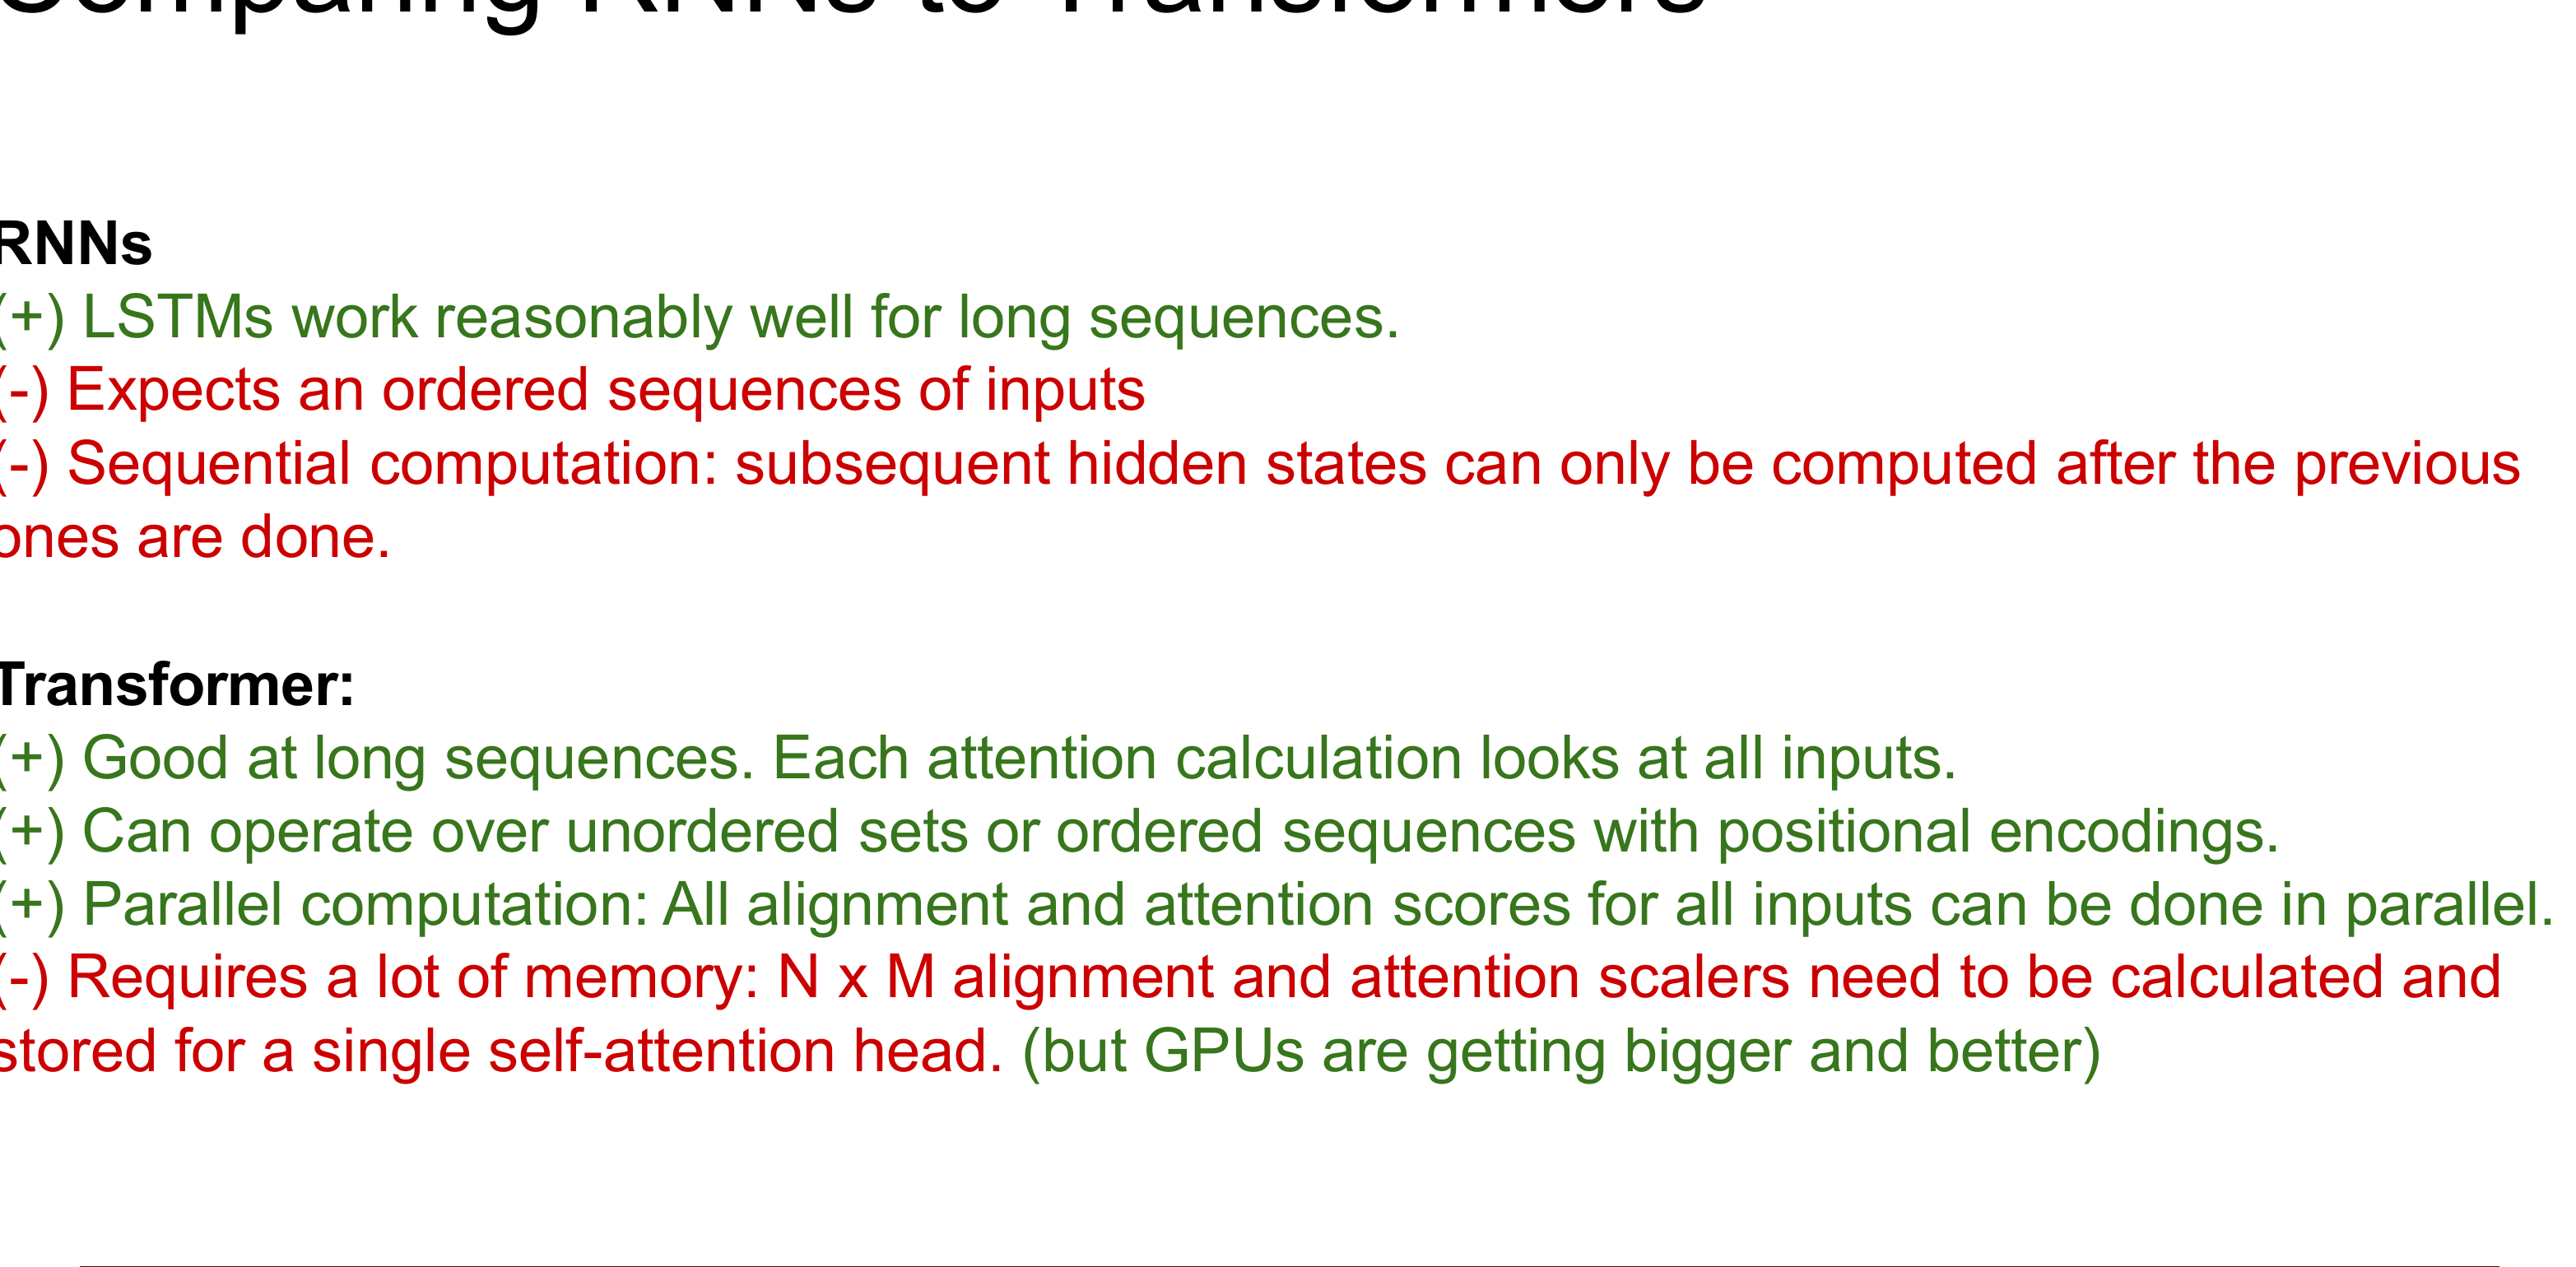
\includegraphics[width=0.90\textwidth]{Pictures/rnn_vs_transformer_table.png}
    \caption{Comparison of RNNs and Transformers (Slide 71). Highlighting parallelization benefits, sequence length handling, and memory trade-offs.}\label{fig:rnn_vs_transformer_table}
\end{figure}

\begin{table}[htbp]
\centering
\small
\renewcommand{\arraystretch}{1.2}
\begin{tabular}{p{0.20\textwidth} p{0.35\textwidth} p{0.35\textwidth}}
\toprule
\textbf{Property} & \textbf{Recurrent Networks (RNN / LSTM)} & \textbf{Transformer Networks} \\
\midrule
\textbf{Temporal Processing} & Strictly sequential ($h_t$ requires $h_{t-1}$). & Fully parallel across all time steps. \\
\textbf{Long-Range Context} & Suffers from exponential signal decay. & Direct $O(1)$ constant path length between any pair. \\
\textbf{Input Structure} & Inherently expects ordered temporal streams. & Operates on unordered sets; order is injected via PE\@. \\
\textbf{Hardware Utilization} & Poor GPU scaling due to sequential loops. & Massive parallel scaling on modern matrix accelerators. \\
\textbf{Memory Footprint} & Linear memory complexity $O(n)$. & Quadratic memory scaling $O(n^2)$ for attention maps. \\
\bottomrule
\end{tabular}
\caption{Comprehensive architectural trade-off comparison between RNNs and Transformers.}\label{tab:rnn_vs_transformer}
\end{table}


\section{Transformers in Computer Vision}

\subsection{Visual Self-Similarity and Non-Local Filtering}

Before Transformers dominated Computer Vision, the core mathematical intuition behind self-attention was widely studied under the concept of \textbf{visual self-similarity}:

\begin{itemize}[leftmargin=*]
    \item \textbf{Self-Similarity in Textures and Natural Images:} As demonstrated by Efros and Leung~\cite{efros1999texture}, natural textures and scenes exhibit pervasive recurring motifs across distant pixel coordinates.
    \item \textbf{Non-Local Means (Buades et al.~\cite{buades2005non}):} In classical image denoising, the Non-Local Means filter updates pixel $i$ by computing a weighted average over all pixels $j$ in the image:
    \begin{equation}
        u(i) = \sum_j w(i, j) v(j), \quad \text{where } w(i, j) \propto \exp\left(-\frac{\|v(N_i) - v(N_j)\|^2}{h^2}\right)
    \end{equation}
    Mathematically, Non-Local Means is identical to self-attention without learnable projections: queries and keys are local image patches, and values are pixel intensities!
\end{itemize}

\subsection{The Evolution of Vision-to-Language Pipelines}

The integration of attention and Transformers progressively transformed vision-to-language models across four distinct generations (Slides 84--86):

\begin{enumerate}[leftmargin=*]
    \item \textbf{CNN + Vanilla RNN (Chapter~\ref{ch:sequence_models}):} A convolutional backbone extracts a single global vector $v$, which initializes a recurrent decoder.
    \item \textbf{CNN + Attentive RNN (Xu et al.~\cite{xu2015show}):} The recurrent decoder dynamically computes 2D spatial attention maps over convolutional feature grids.
    \item \textbf{CNN + Transformer (Image Transformer):} The recurrent language model is replaced with a Transformer decoder, while the visual backbone remains a CNN\@.
    \item \textbf{Pure Transformers (From Pixels to Language):} Convolutions and recurrences are completely removed. The visual image and output text are processed entirely within a unified Transformer architecture.
\end{enumerate}

\subsection{Vision Transformers (ViT)}

Dosovitskiy et al.~\cite{dosovitskiy2020image} proved that pure Transformer architectures could match or surpass Convolutional Networks on large-scale computer vision benchmarks with the introduction of the \textbf{Vision Transformer (ViT)}, illustrated in Figure~\ref{fig:vit_architecture_patches}.

\begin{figure}[htbp]
    \centering
    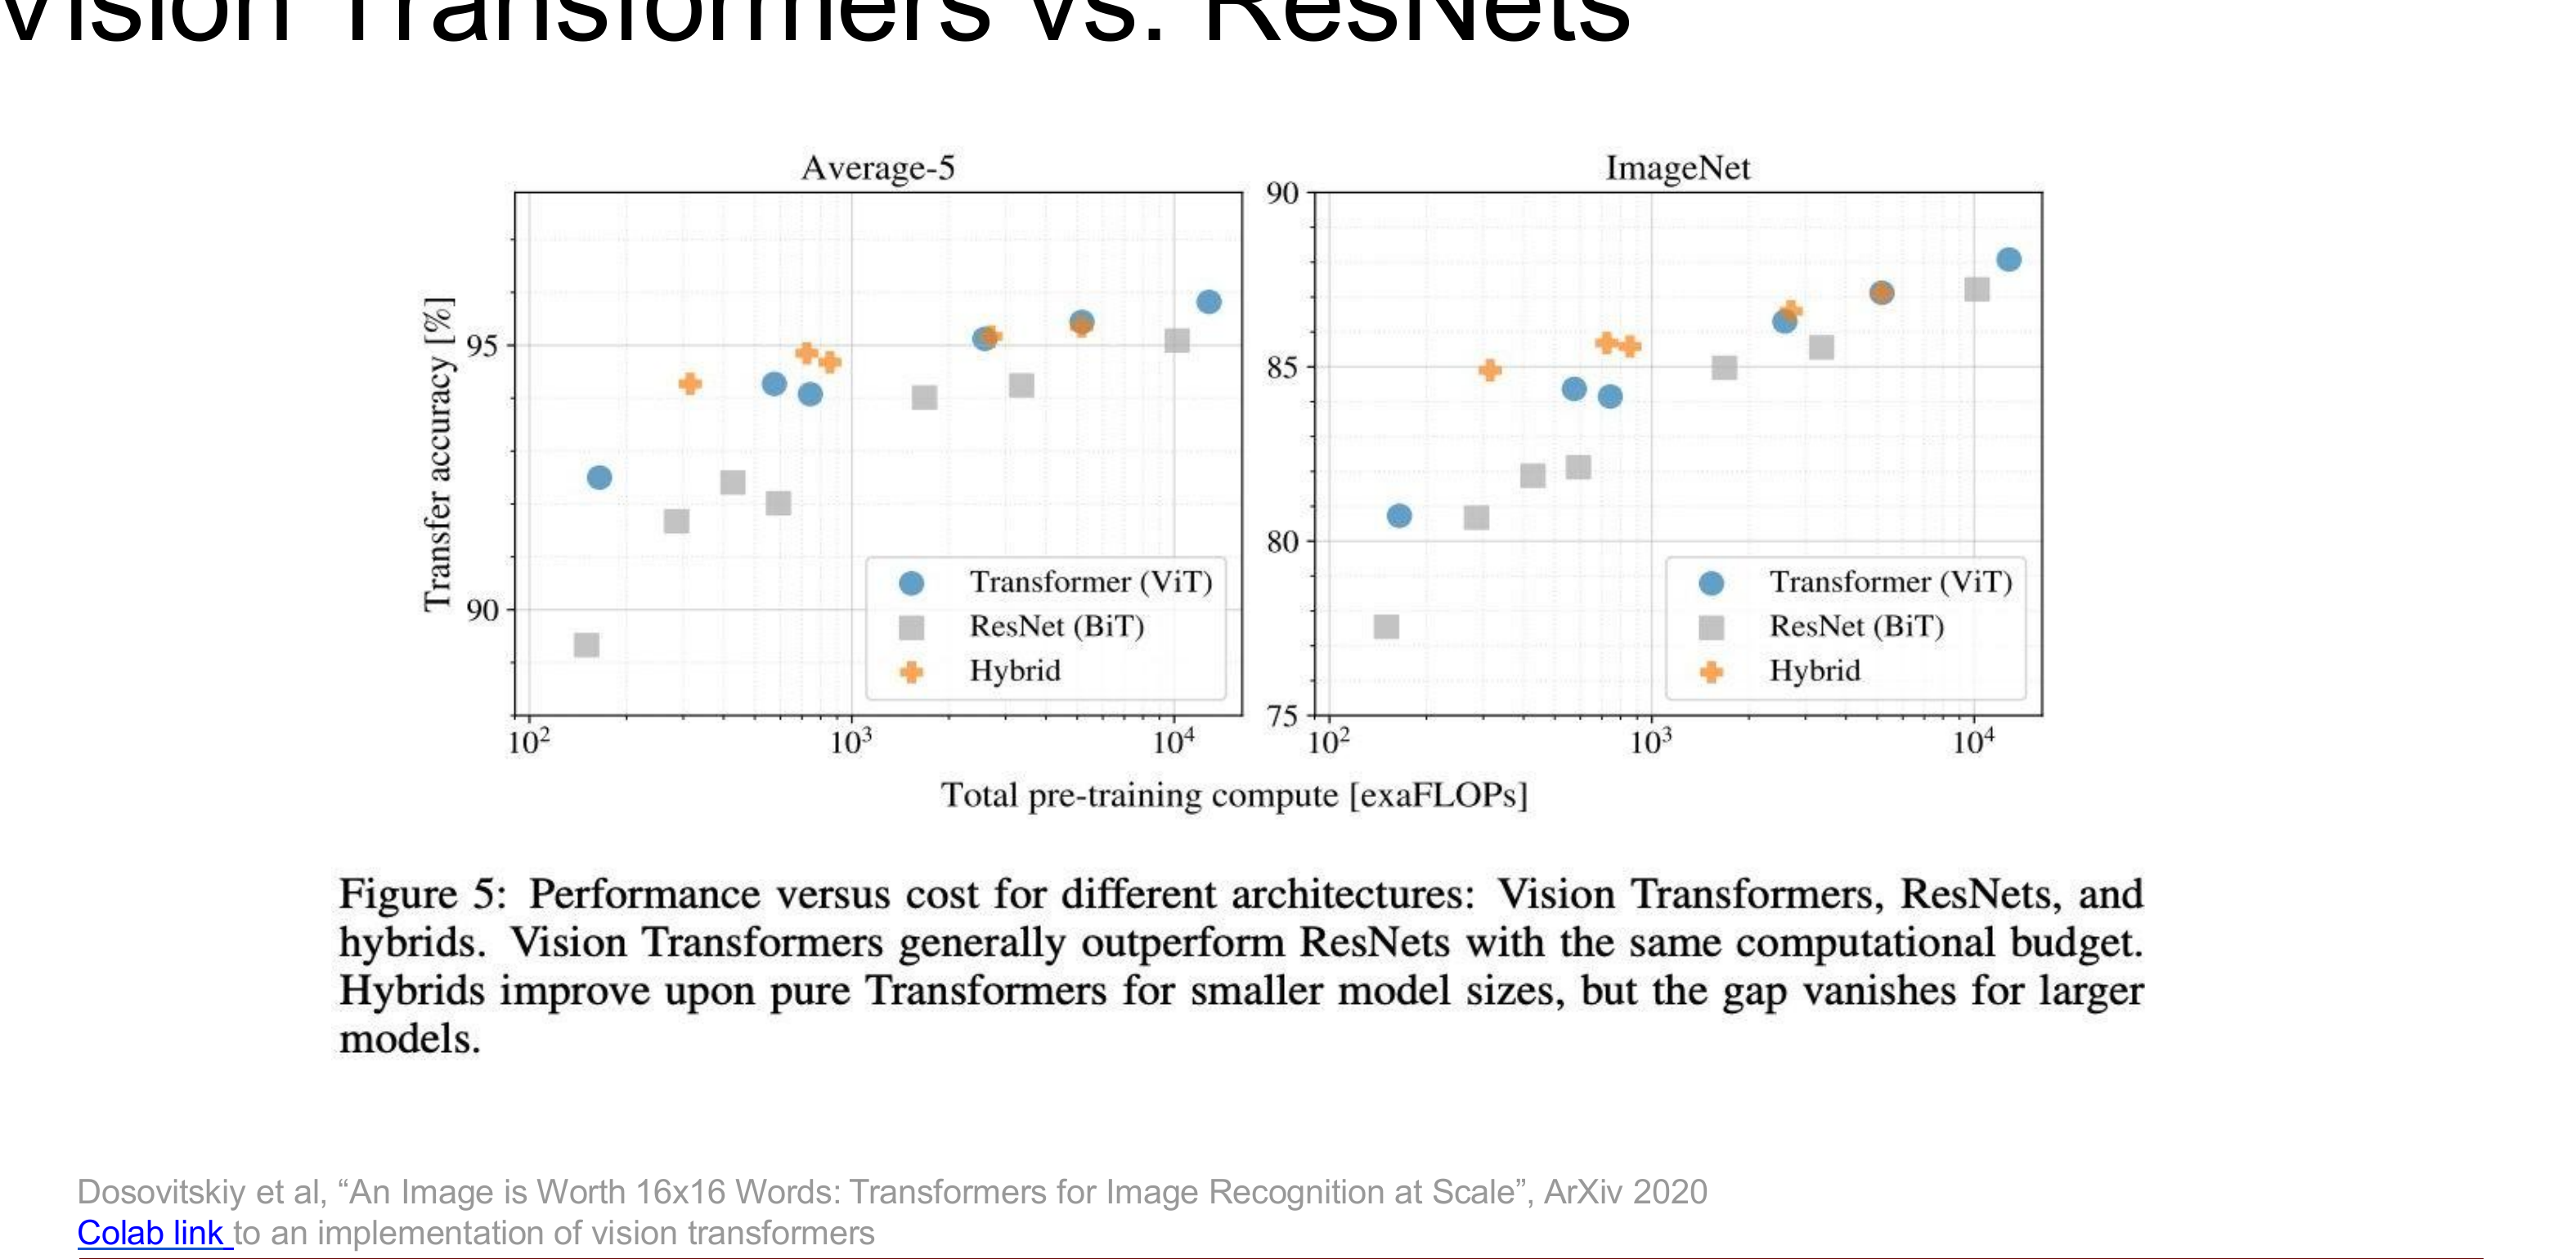
\includegraphics[width=0.90\textwidth]{Pictures/vit_architecture_patches.png}
    \caption{Vision Transformers (ViT) versus ResNets (Dosovitskiy et al.~\cite{dosovitskiy2020image}, from course slides). An image is segmented into $16 \times 16$ non-overlapping patches, linearly projected into embeddings, prepended with a \texttt{[CLS]} token, and processed by a standard Transformer encoder.}\label{fig:vit_architecture_patches}
\end{figure}

The ViT formulation treats image patches as words in a sentence:

\begin{enumerate}[leftmargin=*]
    \item \textbf{Patch Extraction and Linear Embedding:} An image $x \in \mathbb{R}^{H \times W \times C}$ is partitioned into a sequence of $N = \frac{HW}{P^2}$ non-overlapping square patches of size $P \times P$ (typically $P=16$). Each flattened patch $x_p^i \in \mathbb{R}^{P^2 C}$ is linearly projected to dimension $D$ via a trainable embedding matrix $E$:
    \begin{equation}
        z_0 = \left[x_{\text{class}}; \, x_p^1 E; \, x_p^2 E; \, \dots; \, x_p^N E\right] + E_{\text{pos}}
    \end{equation}
    where $E_{\text{pos}} \in \mathbb{R}^{(N+1) \times D}$ is a learnable 1D positional embedding tensor.
    
    \item \textbf{The Classification Token (\texttt{[CLS]}):} Analogous to BERT, a learnable token embedding $x_{\text{class}}$ is prepended to the patch sequence. Because self-attention allows all tokens to interact, the final state of the \texttt{[CLS]} token aggregates global visual context and serves as the input to the classification head.
    
    \item \textbf{Transformer Encoder Stack:} The sequence of $N+1$ token vectors is processed through standard Transformer encoder blocks with Layer Normalization and Multi-Head Self-Attention.
\end{enumerate}

\begin{keywordbox}
\textbf{Inductive Bias: ViT versus ResNet} \\
A central pedagogical takeaway from course Slide 87 is the contrasting nature of their \textbf{inductive biases}:
\begin{itemize}[leftmargin=*]
    \item \textbf{Convnets (ResNets):} Possess strong, hard-coded visual inductive biases: \textbf{two-dimensional locality} (adjacent pixels interact first) and \textbf{translation equivariance} (the same convolution filter operates across all spatial positions).
    \item \textbf{Vision Transformers (ViT):} Have virtually \textbf{zero visual inductive bias}. The model does not inherently know that patch 1 is adjacent to patch 2, nor does it know that patches form a 2D grid; it must learn all geometric relationships from scratch via positional embeddings and attention weights.
\end{itemize}
\textbf{The Scaling Regime:}
Because ViT has little inductive bias, when trained on small or medium datasets (e.g., ImageNet-1K with 1.3M images), it tends to overfit and performs worse than ResNet. However, when pre-trained on massive datasets (such as Google's JFT-300M with 300 million images), ViT's superior capacity and global receptive field from layer 1 decisively outperform ResNets!
\end{keywordbox}

Modern hierarchical adaptations have since generalized ViTs to multi-scale vision tasks:
\begin{itemize}[leftmargin=*]
    \item \textbf{DETR (Carion et al.~\cite{carion2020end}):} Treats object detection as a direct set-prediction problem using Transformer encoder-decoders and bipartite Hungarian matching, eliminating anchor boxes and Non-Maximum Suppression (NMS).
    \item \textbf{Swin Transformer (Liu et al.~\cite{liu2021swin}):} Computes self-attention within local shifted windows, reducing computational complexity from quadratic $O({(HW)}^2)$ to linear $O(HW)$ while preserving multi-scale feature hierarchies suitable for dense segmentation.
    \item \textbf{Multiscale Vision Transformers (MViT) (Fan et al.~\cite{fan2021multiscale}):} Progressively reduces spatial resolution while expanding channel dimensions across stages, optimizing compute for high-resolution video and image recognition.
\end{itemize}


\section{Pre-training, BERT, and Model Compression}

\subsection{The ``ImageNet Moment'' for Natural Language Processing}

In Computer Vision, transfer learning using ImageNet pre-training had been the gold standard since AlexNet (Chapter~\ref{ch:convnets}). For years, Natural Language Processing lacked an equivalent universal pre-training paradigm, relying instead on shallow static embeddings (Word2Vec, GloVe).

In 2018, the Transformer enabled the true \textbf{``ImageNet Moment for NLP''} (Slide 62):
\begin{enumerate}[nosep, leftmargin=*]
    \item \textbf{Pre-training Phase:} Train a massive Transformer model on hundreds of gigabytes of unannotated text scraped from the internet using self-supervised objectives.
    \item \textbf{Fine-Tuning Phase:} Adapt the pre-trained weights to specific downstream tasks (classification, question answering, named entity recognition) with a small task-specific head, requiring minimal labeled data.
\end{enumerate}

\subsection{\texorpdfstring{BERT:}{BERT:} Bidirectional Encoder Representations from Transformers}

Prior pre-trained models (such as OpenAI GPT) relied on standard autoregressive language modeling: predicting token $x_t$ given left-to-right context $x_{<t}$. However, language understanding is intrinsically \textbf{bidirectional}: words derive their meaning from both preceding and succeeding context.

\begin{figure}[htbp]
    \centering
    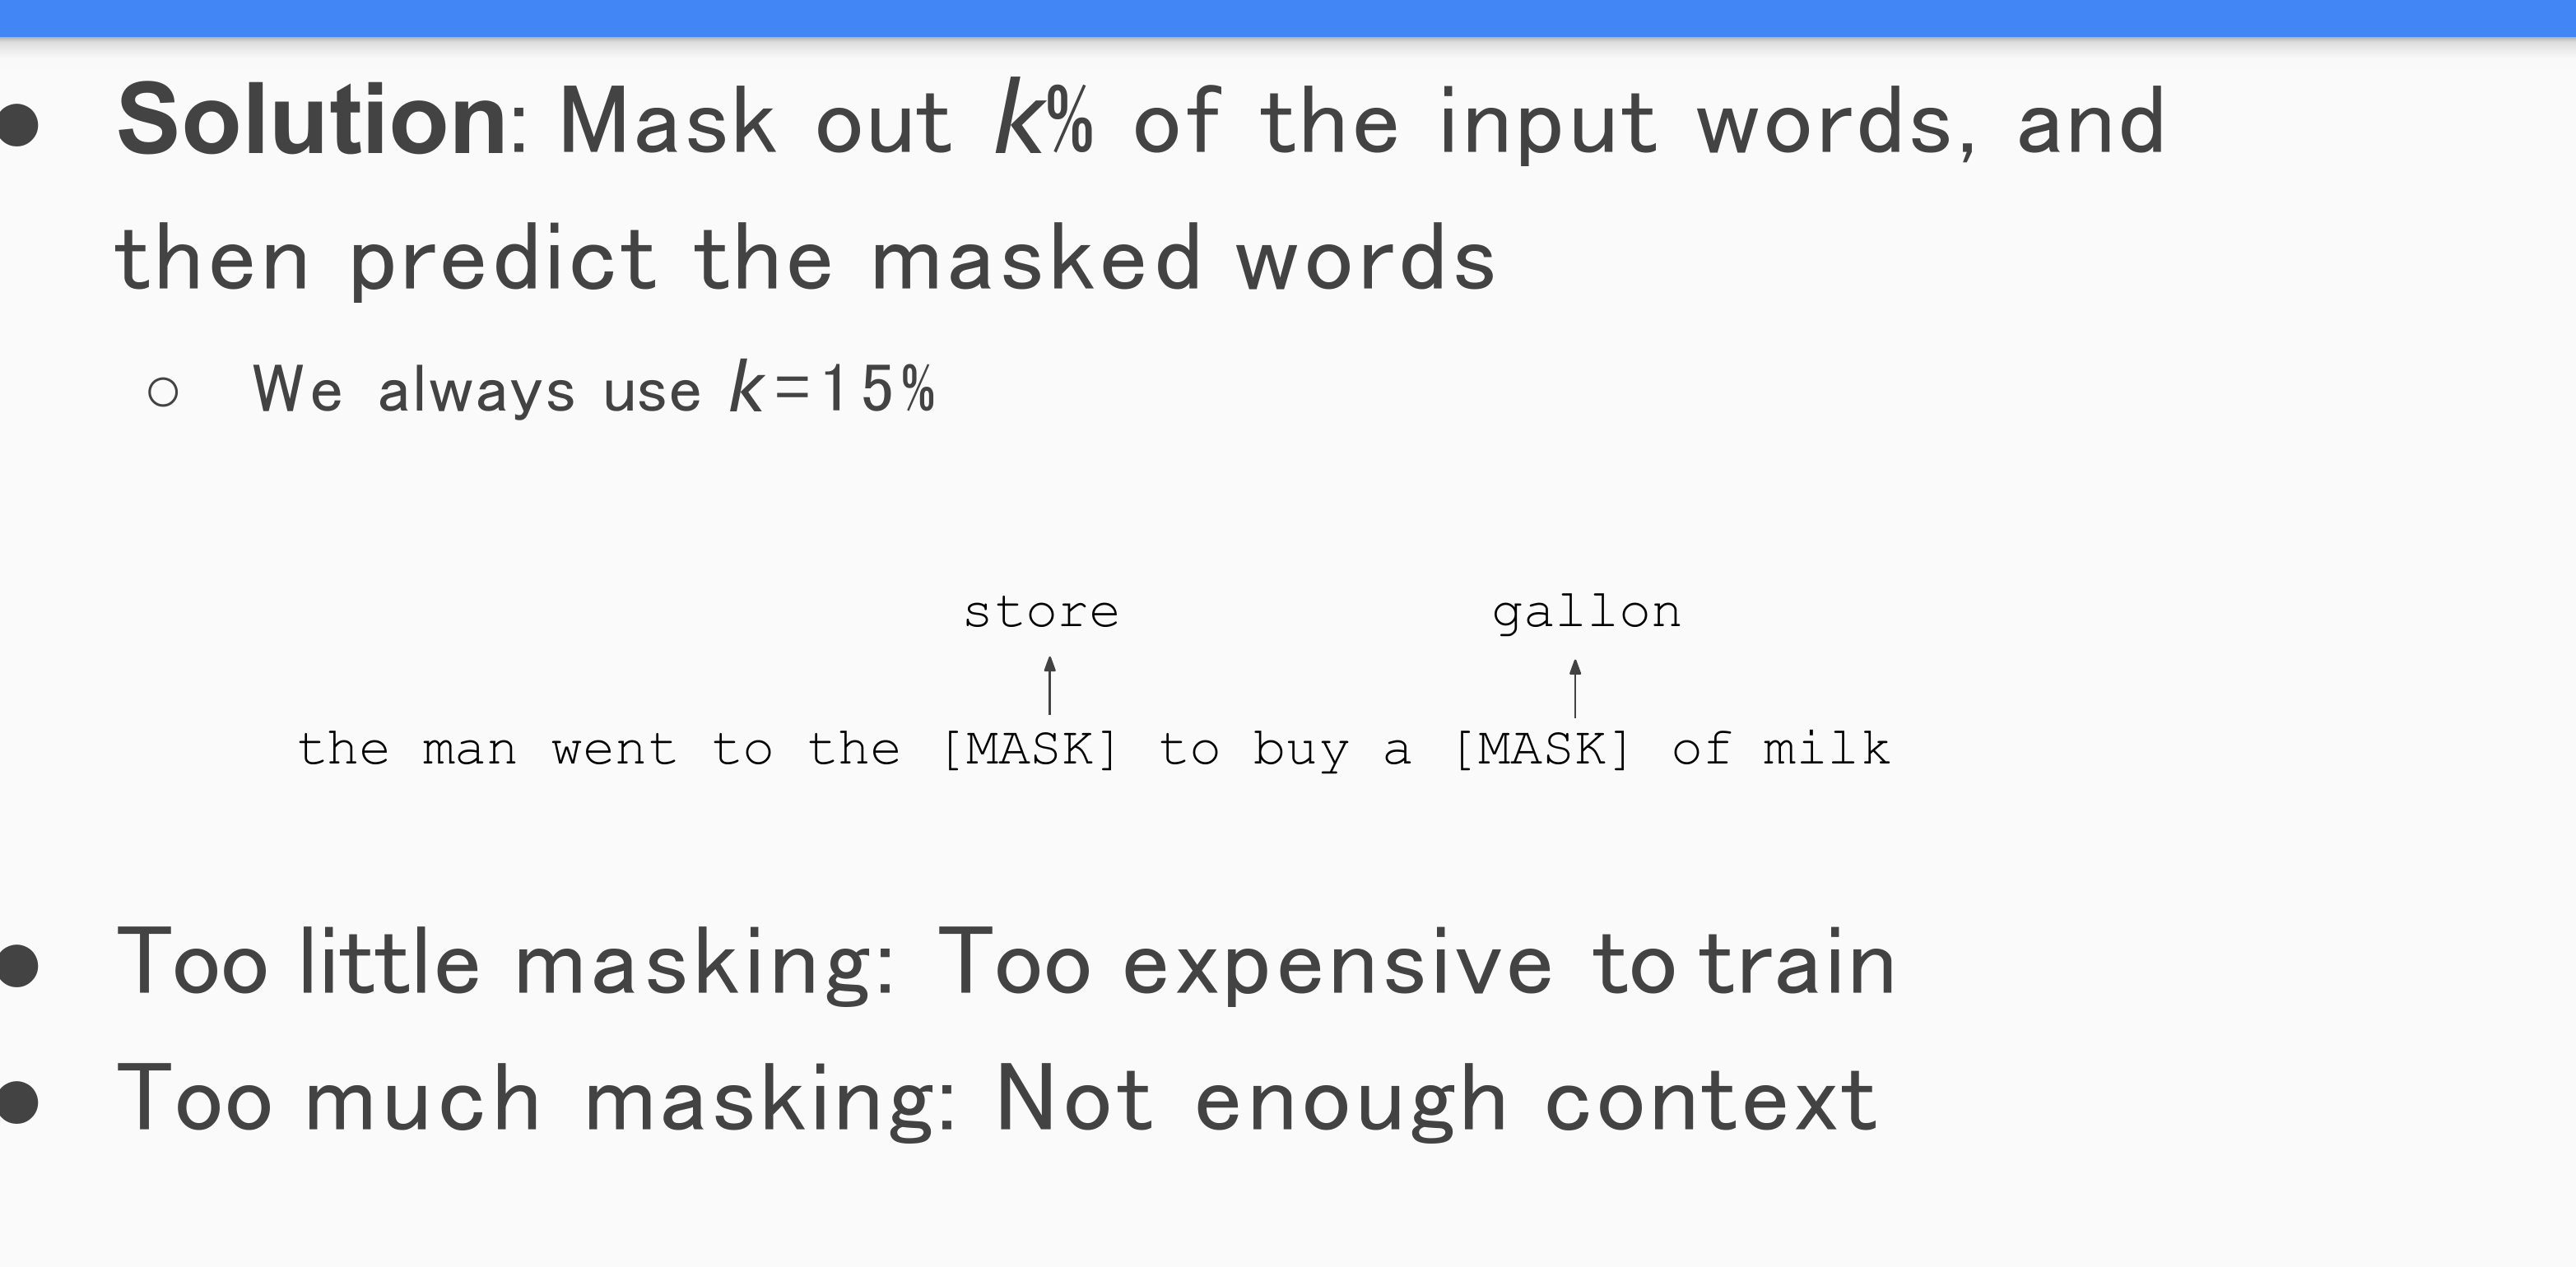
\includegraphics[width=0.88\textwidth]{Pictures/bert_masked_lm_pretraining.png}
    \caption{BERT Masked Language Model (MLM) pre-training (Devlin et al.~\cite{devlin2019bert}, from course slides). 15\% of input tokens are masked, and the model predicts the original words using full bidirectional context.}\label{fig:bert_masked_lm_pretraining}
\end{figure}

Why could standard language models not be bidirectional? In a multi-layer bidirectional Transformer, tokens in upper layers would trivially “see themselves” through intermediate connections, reducing the next-word prediction task to trivial copying.

To solve this dilemma, Devlin et al.~\cite{devlin2019bert} introduced \textbf{BERT} and the \textbf{Masked Language Model (MLM)} objective, illustrated in Figure~\ref{fig:bert_masked_lm_pretraining}:

\begin{enumerate}[leftmargin=*]
    \item \textbf{15\% Masking Rule:} Exactly 15\% of the input tokens are chosen at random. Of these chosen tokens:
    \begin{itemize}[nosep]
        \item 80\% are replaced with the special mask token \texttt{[MASK]}.
        \item 10\% are replaced with a random word.
        \item 10\% are kept unchanged.
    \end{itemize}
    \item \textbf{Bidirectional Context Processing:} The corrupted sequence is fed through a deep Transformer encoder, where every token attends freely to all other tokens in both directions.
    \item \textbf{Selective Cross-Entropy Loss:} A classification head over the vocabulary predicts the original identity of the masked tokens. The training loss considers \textbf{only} the predictions at the masked positions:
    \begin{equation}
        L_{\text{MLM}} = -\sum_{i \in \text{masked}} \log P(x_i | \widetilde{X})
    \end{equation}
\end{enumerate}

\begin{Notebox}
\textbf{Why Exactly 15\% Masking?} \\
Course Slide 92 emphasizes this fundamental optimization trade-off:
\begin{itemize}[nosep, leftmargin=*]
    \item \textit{Too little masking ($< 15\%$):} Too few gradient signals are generated per sentence, making pre-training excessively slow and computationally prohibitive.
    \item \textit{Too much masking ($> 15\%$):} Insufficient contextual clues remain in the corrupted sentence, preventing the network from learning meaningful syntactic and semantic dependencies.
\end{itemize}
\end{Notebox}

Alongside MLM, BERT was trained on a secondary objective: \textbf{Next Sentence Prediction (NSP)}, where the model predicts whether two paired input sentences appeared consecutively in the original text or were randomly paired.

\subsection{\texorpdfstring{ELECTRA:}{ELECTRA:} Efficient Pre-training as Discriminators}

While BERT achieved state-of-the-art results, computing loss on only 15\% of tokens represents substantial sample inefficiency. Clark et al.~\cite{clark2020electra} resolved this limitation with \textbf{ELECTRA}, training text encoders as \textbf{discriminators} rather than generators.

\begin{keywordbox}
\textbf{Replaced Token Detection (RTD)} \\
ELECTRA consists of two networks trained jointly:
\begin{enumerate}[nosep, leftmargin=*]
    \item \textbf{Generator (Small MLM):} Predicts masked tokens in the standard 15\% corrupted sequence, producing plausible word substitutions.
    \item \textbf{Discriminator (Target Transformer Encoder):} Instead of predicting word identities over a 30,000-word vocabulary, the discriminator solves a binary classification task for \textbf{every single token}: predicting whether each token is \textbf{original} or has been \textbf{replaced} by the generator.
\end{enumerate}
\textbf{Key Advantage:}
Because binary classification is evaluated over the entire sequence, \textbf{100\% of the tokens contribute to the loss gradient} at every step (rather than just 15\% in BERT). Consequently, ELECTRA achieves comparable or superior downstream accuracy with less than $25\%$ of BERT's training compute.
\end{keywordbox}

\subsection{Knowledge Distillation and Model Compression}

While massive Transformer models achieve outstanding accuracy, their billions of parameters introduce prohibitive latency and memory footprints, hindering deployment in real-time edge devices and low-latency production microservices.

Course Slide 99 highlights the primary technique for solving this operational bottleneck: \textbf{Knowledge Distillation} (pioneered by Bucil{\u{a}} et al.~\cite{bucila2006model}, Hinton et al.~\cite{hinton2015distilling}, and extended to adversarial compression by Belagiannis, Farshad, and Galasso~\cite{belagiannis2018adversarial}).

\begin{figure}[htbp]
    \centering
    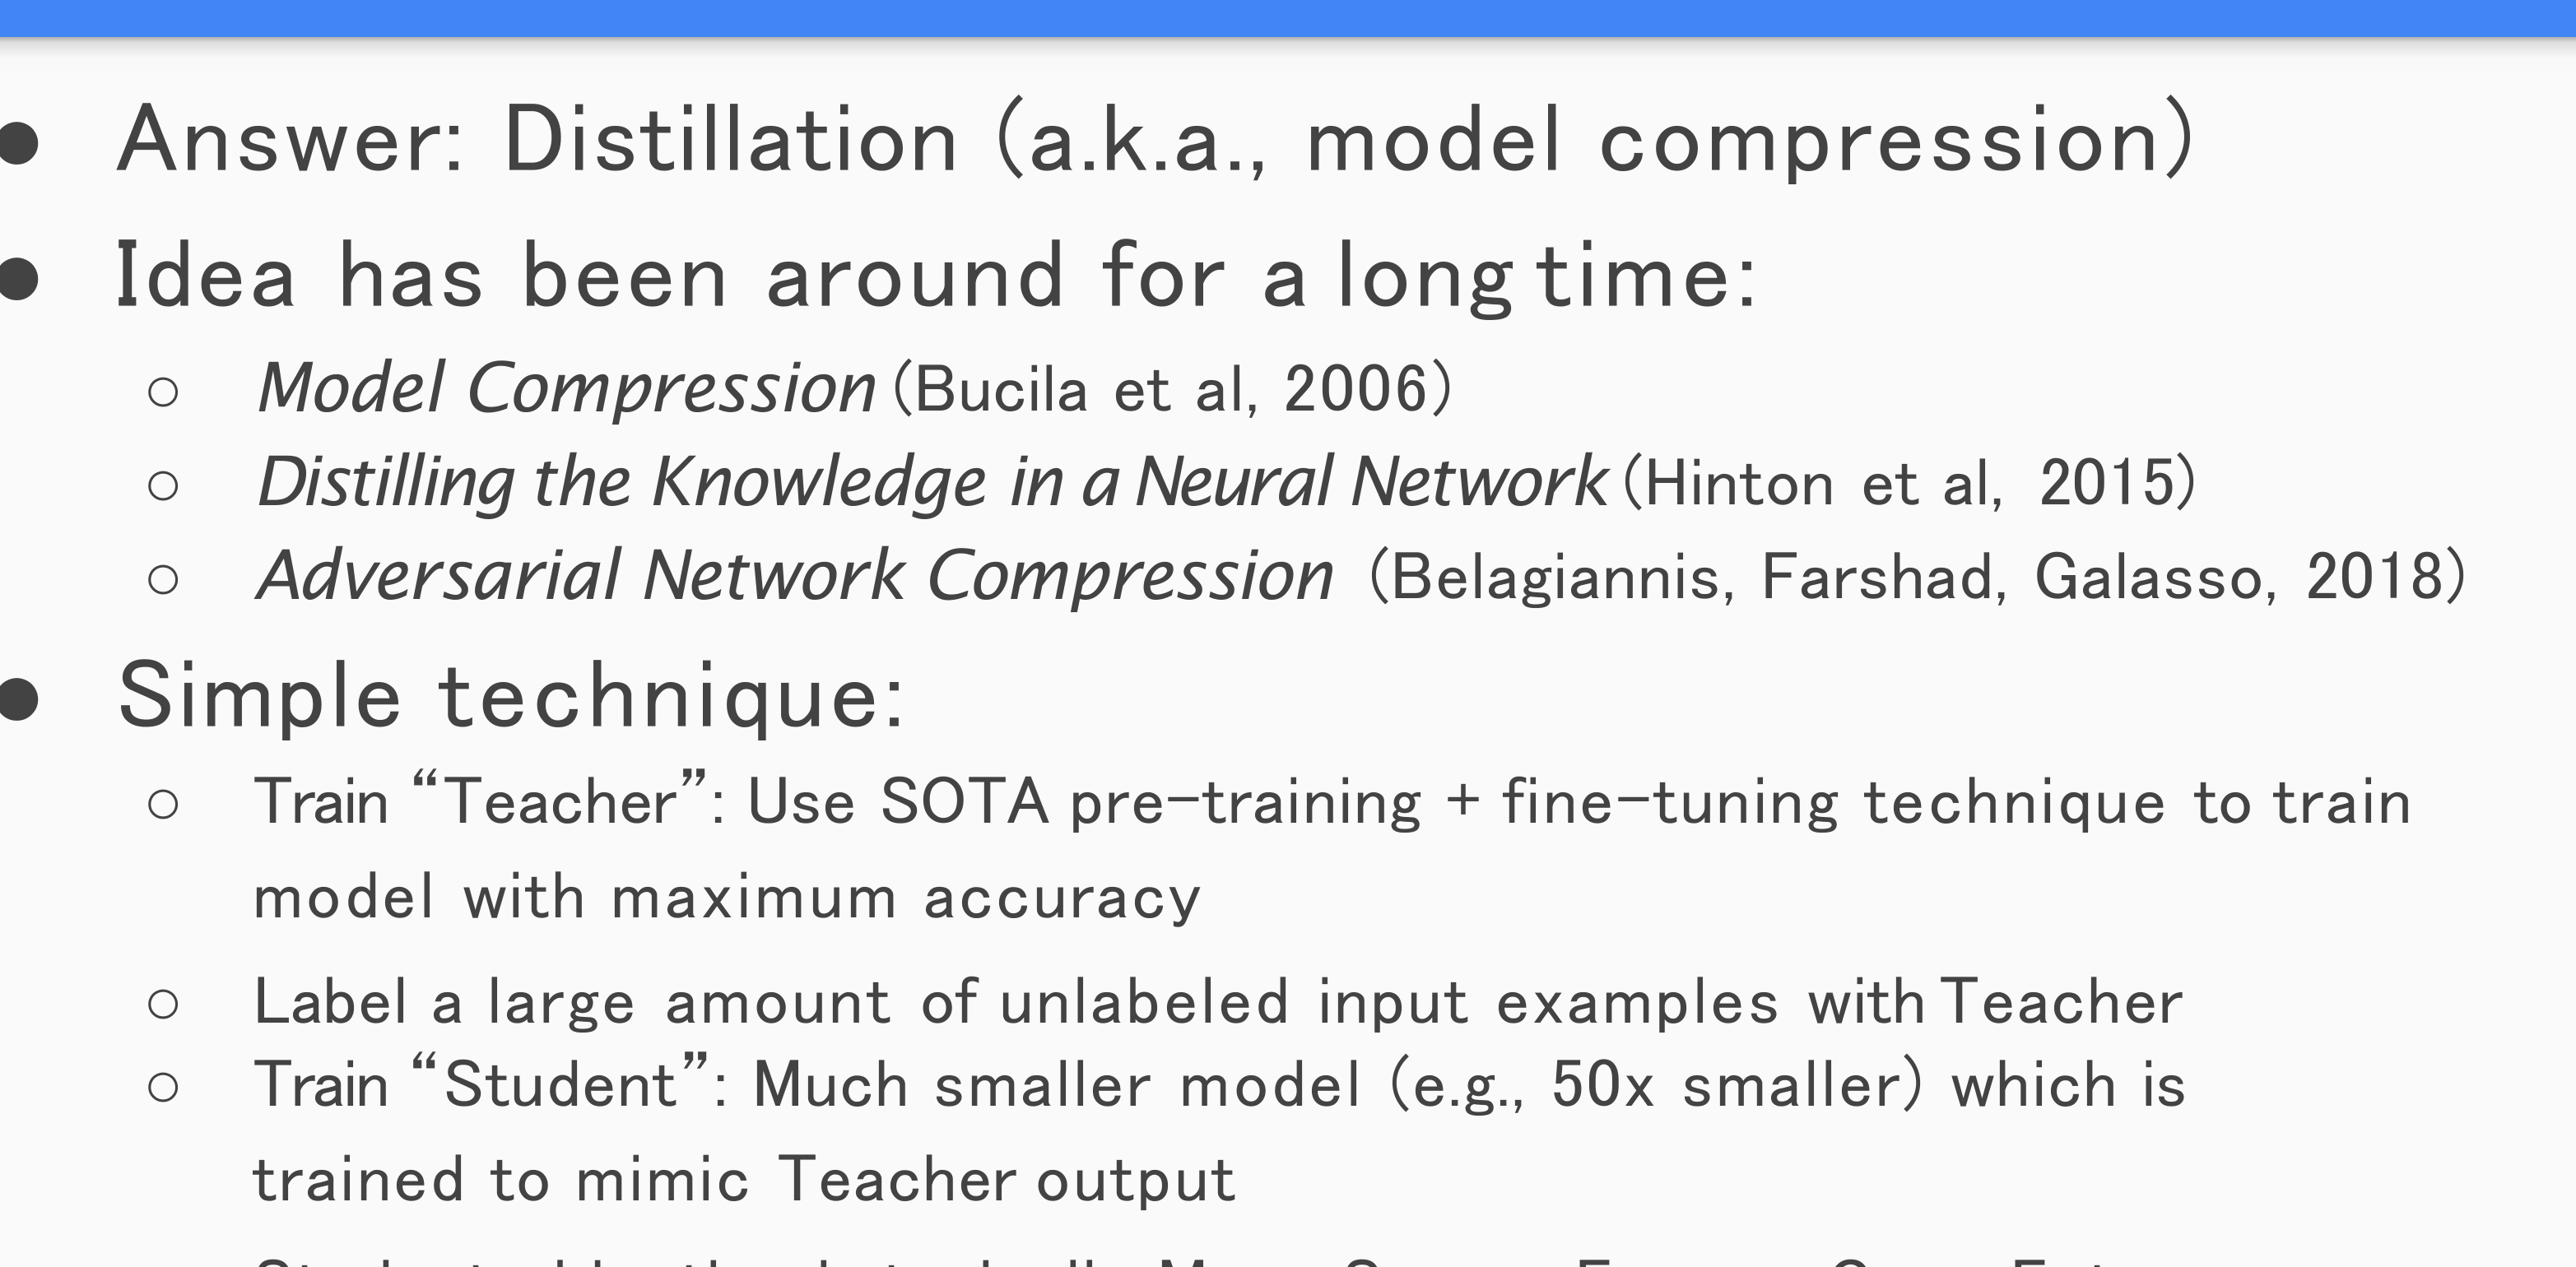
\includegraphics[width=0.88\textwidth]{Pictures/knowledge_distillation_teacher.png}
    \caption{Knowledge Distillation for Transformer model compression (Slide 99). A high-capacity Teacher network generates soft probability distributions over unlabeled data, supervising a compact Student model.}\label{fig:knowledge_distillation_teacher}
\end{figure}

The distillation protocol proceeds through three distinct phases:
\begin{enumerate}[leftmargin=*]
    \item \textbf{Train the Teacher Network:} A large, high-capacity Transformer (e.g., BERT-Large) is trained using standard pre-training and task fine-tuning to achieve maximum accuracy.
    \item \textbf{Soft Target Generation:} The frozen Teacher evaluates a massive corpus of unlabeled data, generating soft probability distributions over classes:
    \begin{equation}
        q_i = \frac{\exp(z_i / T)}{\sum_j \exp(z_j / T)}
    \end{equation}
    where $T > 1$ is the distillation \textbf{temperature}, which softens output distributions to reveal the \textit{``dark knowledge''} (relative probabilities assigned to incorrect classes).
    \item \textbf{Train the Student Network:} A much smaller Student model (e.g., 50x smaller, such as DistilBERT or compact BERT~\cite{turc2019well}) is trained to mimic the Teacher's soft outputs by minimizing Kullback-Leibler (KL) divergence or Cross-Entropy:
    \begin{equation}
        L_{\text{distill}} = \alpha L_{\text{hard}}(y_{\text{student}}, y_{\text{true}}) + (1 - \alpha) T^2 \operatorname{KL}\left(q_{\text{student}} \,\|\, q_{\text{teacher}}\right)
    \end{equation}
\end{enumerate}

Empirically (Slide 100), distilling a Teacher into a smaller model yields substantially higher accuracy than training the smaller model from scratch directly on labeled data. Knowledge distillation allows production systems to retain over 97\% of BERT's performance while operating at a fraction of the inference latency.


\newpage
\section{Chapter Summary and Conceptual Graph}

The concepts developed in this chapter establish the architectural foundations of modern attention and Transformer networks, tracing the path from recurrent bottlenecks to pure attention and self-supervised foundation models:

\begin{InsightBox}
\textbf{The Logical Connections Between Nodes:}
\begin{itemize}[leftmargin=*]
    \item \textbf{From Node 1 to 2:} The fixed-dimensional bottleneck vector $c=h_T$ of Vanilla Seq2Seq degrades on long sequences; Bahdanau attention resolves this by computing dynamic, content-based alignments $c_t = \sum_i \alpha_{t,i} h_i$.
    \item \textbf{From Node 2 to 3:} Recognizing that attention operates over unordered sets allows extending attention to spatial 2D convolutional grids, enabling models to dynamically focus on image regions during caption generation.
    \item \textbf{From Node 3 to 4:} Eliminating recurrent transitions entirely, Self-Attention allows tokens within the same sequence to interact directly via Queries, Keys, and Values with a constant $O(1)$ maximum path length.
    \item \textbf{From Node 4 to 5:} Because self-attention is permutation equivariant, Positional Encodings (sinusoidal or learned) are added to inject temporal ordering, while Causal Masking ($-\infty$) enforces autoregressive validity in parallel.
    \item \textbf{From Node 5 to 6:} Wrapping Multi-Head Self-Attention with residual connections, Layer Normalization, and point-wise MLPs creates the complete Transformer Encoder and Decoder blocks.
    \item \textbf{From Node 6 to 7:} Partitioning images into $16 \times 16$ patches translates 2D vision into token sequences, enabling Vision Transformers (ViT) to outperform ResNets at scale despite minimal hard-coded inductive biases.
    \item \textbf{From Node 7 to 8:} Transformers unlock massive self-supervised pre-training via Masked Language Modeling (BERT) and discriminative Replaced Token Detection (ELECTRA), with Knowledge Distillation enabling real-time production deployment.
\end{itemize}
\end{InsightBox}

\begin{figure}[htbp]
\centering
\begin{tikzpicture}[
    node distance=0.55cm and 0cm,
    conceptnode/.style={
        rectangle, rounded corners=4pt, draw=ocre!80, fill=ocre!8,
        line width=0.8pt, text width=0.88\textwidth, inner sep=4.5pt,
        font=\sffamily\small
    },
    arrowline/.style={
        ->, >=Stealth, line width=1pt, color=ocre!80
    }
]

\node[conceptnode] (n1) {\textbf{1. Vanilla Seq2Seq Information Bottleneck}\\
Compressing sequences into a single static context vector $c=h_T$ causes catastrophic forgetting on long horizons.};

\node[conceptnode, below=of n1] (n2) {\textbf{2. Bahdanau Additive Attention}\\
Computes scalar alignments $e_{t,i}$ and Softmax weights $\alpha_{t,i}$, generating dynamic context vectors $c_t$ over unordered sets.};

\node[conceptnode, below=of n2] (n3) {\textbf{3. Spatial Attention in Computer Vision}\\
Applies 2D attention over convolutional feature maps $z \in \mathbb{R}^{H \times W \times D}$ (\textit{Show, Attend and Tell}), focusing on salient visual regions.};

\node[conceptnode, below=of n3] (n4) {\textbf{4. Self-Attention \& Scaled Dot-Product ($Q, K, V$)}\\
All-to-all token interactions with $O(1)$ path length; scaling by $1/\sqrt{D_k}$ prevents Softmax gradient saturation.};

\node[conceptnode, below=of n4] (n5) {\textbf{5. Positional Encoding, Causal Masking \& Multi-Head}\\
Sinusoidal encodings break permutation equivariance; causal $-\infty$ masking enables parallel training; multi-head mimics conv filter banks.};

\node[conceptnode, below=of n5] (n6) {\textbf{6. The Full Transformer Architecture}\\
Encoder and Decoder stacks combining Multi-Head Attention, Cross-Attention, Residual Connections, and Layer Normalization.};

\node[conceptnode, below=of n6] (n7) {\textbf{7. Vision Transformers (ViT)}\\
Splits images into $16 \times 16$ patches; trades off inductive biases for massive global capacity, outperforming ResNets at scale.};

\node[conceptnode, below=of n7] (n8) {\textbf{8. Pre-training, BERT, ELECTRA \& Distillation}\\
Self-supervised Masked LM, discriminative Replaced Token Detection, and Teacher-Student compression for efficient deployment.};

\draw[arrowline] (n1) -- (n2);
\draw[arrowline] (n2) -- (n3);
\draw[arrowline] (n3) -- (n4);
\draw[arrowline] (n4) -- (n5);
\draw[arrowline] (n5) -- (n6);
\draw[arrowline] (n6) -- (n7);
\draw[arrowline] (n7) -- (n8);

\end{tikzpicture}
\caption{Conceptual roadmap of Attention Mechanisms, Transformer Networks, ViT, and Pre-training.}\label{fig:ch4_roadmap}
\end{figure}
